% ---------------
% PREAMBLE
% ---------------
\documentclass[tagged,twocolumn]{CorporateReport}

% -----------------------------------
% DOCUMENT PROPERTIES
% -----------------------------------
\title{Writing Corporate Documents using LaTeX}
\author{A. Clifton}
\addbibresource{files/bibliography.bib}

% -------------------------------------
% DOCUMENT STARTS HERE
% -------------------------------------
\begin{document}

\frontmatter
\chapter*{Executive Summary}
This document is a guide to writing documents for publication by NREL using the LaTeX document preparation system. LaTeX is not WYSIWYG and has different reviewing and editing tools compared to typical word processing software. For this reason special care has to be taken when preparing NREL documents in LaTeX. This document serves both as a guide to implementing NREL's style and formatting guidelines in LaTeX, and as a template. This document is intended for people with some familiarity with LaTeX.
\chapter*{Acknowledgments}
This document and the NREL LaTeX class file were developed by staff at the National Wind Technology Center, including Andrew Platt, Andrew Clifton, Andrew Ning, Mike Lawson, and Paul Fleming. Alexsandra Lemke provided support relating to NREL communications. A first demonstration of an NREL class file was created by Chuck Booten from NREL's Electricity, Resources, and Building Systems Integration group, which inspired this effort. The class file and this template were developed as part of work on several NREL reports, journal articles, and conference publications. 

We thank members of the TeX -- LaTeX StackExchange site for useful suggestions concerning LaTeX and typography \cite{texstackexchange}.

This report was typeset using the LaTeX typesetting system originally developed by Leslie Lamport, based on TeX created by Donald Knuth.

\mainmatter
\tableofcontents
\listoffigures
\listoftables

\lstset{language=[LaTeX]Tex,columns=fullflexible,keepspaces=true,breaklines=true}
%% CHAPTER: WHAT IS LATEX
\chapter{What is LaTeX?}
LaTeX is a mark-up language that describes how a document should be prepared. Three things are needed to make a LaTeX document:
\begin{enumerate}
\item A source document, usually with extension \emph{.tex}
\item Some packages and classes that help turn what's in the source document into something helpful
\item A compiler, also referred to as a working LaTeX installation.
\end{enumerate}

At first glance the source document looks like a programming language, and that's because it is: LaTeX is not WYSIWYG, like many of the document preparation tools in common use today. A good analogy is html.

\section{Printed Resources}


\section{Online Resources}
The wikibook at \href{http://en.wikibooks.org/wiki/LaTeX}{http://en.wikibooks.org/wiki/LaTeX} is an excellent resource. There are also several internet forums such as \href{tex.stackexchange.com}{tex.stackexchange.com} that may be useful.

Documentation for the packages used in the nrel.cls file (Section \ref{sec:nrelcls}) can be found at \href{ctan.org}{ctan.org}.

%% CHAPTER: HOW TO MAKE LATEX DOCUMENTS %%
\section{Using LaTeX to Make Corporate Documents }
A series of LaTeX class files called \emph{Corporate...cls} have been written to implement common formatting requirements in LaTeX.

\subsection{Corporate class files}\label{sec:Corporatecls}
Class files control the formatting and presentation of documents. The class files currently available include:
\begin{description}
\item[CorporateReport.cls]{compiles the document using the LaTeX \emph{report} class, with corporate formatting. This is intended for longer documents and allows the use of chapters.}
\item[CorporateArticle.cls] compiles the document using the LaTeX \emph{article} class, with corporate formatting. This is intended for shorter documents such as journal articles. This class does not support the use of chapters.
\item[CorporateResources.tex] contains the common packages and formatting descriptions that are implemented by the \emph{CorporateReport.cls} and \emph{CorporateArticle.cls} classes.
\end{description}

As with normal classes, options are passed to the class in the \verb+\documentclass+ line:

\begin{lstlisting}
\documentclass[option1,...,optionn]{CorporateArticle}
\end{lstlisting}

Options specific to \emph{Corporate*.cls} include:
\begin{description}
\item[draft]{add a `draft' watermark to all pages.}
\end{description}

The \emph{Corporate....cls} files call a variety of other packages. Packages are codes that modify the appearance or behaviour of LaTeX to achieve something. Table \ref{Tab:Packages} lists the packages that are explicitly called by \emph{Corporate*.cls} or \emph{CorporateResources.tex} in the order they are called in. These packages often call other packages, so this is not an exhaustive list.

\begin{table*}[!h]
\centering
\caption[Packages loaded by the Corporate classes]{Packages loaded by the Corporate classes.}
\label{Tab:Packages}
\begin{tabular*}{\textwidth}{llp{0.6\textwidth}}
\toprule
Package & Options & Functionality\\
\midrule
%accessibility & tagged & generates the document structure and tagging \\
amsfonts, amssymb & & supplies AMS fonts, which are useful for mathematics \\
babel & english & activates language-appropriate hyphenation rules\\
booktabs & & improves the formatting of tables \\
caption & & required to generate captions for floats\\
fontenc & T1 & enables direct typing of international characters \\
geometry & & sets page size and margins \\
graphicx & & graphics handling, including \emph{.eps} figures \\
hyphenat & & improves spacing and breaking of hyphenated words \\
listings & & enables the inclusion of high-quality computer code listings\\
nag & & checks that packages are up to date and looks for bad habits in LaTeX code. \\
parskip & & required for better spacing\\
pdfcomment & & required for tool-tips. Also calls the \texttt{hyperref} package  \\
setspace & & required for better spacing\\
subcaption & & provides the \texttt{subfigure} environment to produce sub figures \\
tocloft & & improved table of contents and list of figures/tables in memoir documents\\
tocbibind & nottoc, notlot, notlof & Add bibliography/index/contents to Table of Contents in memoir documents\\
todonotes & & inline and margin to-do notes \\
xcolor & & Driver-independent color extensions for LaTeX and pdfLaTeX\\
\bottomrule
\end{tabular*}
\end{table*}

It should be noted that the `english` option to Babel really means \emph{American} English.

\subsubsection{Starting new documents}
\begin{enumerate}
\item Go to \href{https://github.com/xx}{https://github.com/xx} and download the latest version of the repository as a .zip file from the icon on the lower right hand side of the page.
\item ...
\item Modify \emph{main.tex} as required.
\end{enumerate}

\subsection{Creating Content}
\subsubsection{Front, main, and back matter}
The convention in this corporate class is to have Roman numerals in the front matter, and then arabic numerals in the main matter of the document (after the tables of contents, figures and tables). Tables and figures in the front matter are also numbered differently (Table A, B, C, ...) than in the main matter (Table 1, 2, 3, ...).

This change in page and float numbering is implemented using the \verb+\frontmatter+, \verb+\mainmatter+, and \verb+\backmatter+ commands at the start of these sections of the document:

\begin{lstlisting}
\begin{document}

\maketitle
\frontmatter
...
\tableofcontents
\clearpage
\listoffigures
\listoftables
\mainmatter
...
\backmatter
\end{document}
\end{lstlisting}

Page numbering in the front matter (i.e. the Abstract, Summary, and Foreword chapters or sections) starts at page 3 to allow for cover pages.

If you don't use the \verb+\frontmatter+ commands, you may need to increment the page counter manually. To increment the counter $n$ pages, use \verb+\setcounter{page}{n}+ after \verb+\begin{document}+.

\subsubsection{Cross references}
Use labels and references to refer back and forth to figures, equations, tables and sections. 

For example, an equation can be added using the following text:

\begin{lstlisting}
\begin{equation}
y = mx+c
\label{eqn:line}
\end{equation}
\end{lstlisting}

This gives the following:
\begin{equation}
y = mx+c
\label{eqn:line}
\end{equation}

And using the text \verb+Eqn. \ref{eqn:line}+ provides a cross reference to Eqn. \ref{eqn:line}.

\subsubsection{Floats}
Floats are images, tables or other pieces of the document that are free to move to the best place in the document for them. The two most common floats are the tabular environment (for tables) and the figure environment for figures.

\paragraph{Tables}
Use the \texttt{tabular} environment to produce basic tables. Table~\ref{tab:widgets} is produced using this code: 

\begin{lstlisting}
\begin{table}[!h]
\centering
\caption{An example table.}\label{tab:widgets}
\begin{tabular}{lr}
Item & Quantity \\
\hline
Widgets & 42 \\
Gadgets & 13
\end{tabular}
\end{table}
\end{lstlisting}

\begin{table}[!h]
\centering
\caption{An example table.}\label{tab:widgets}
\begin{tabular}{lr}
Item & Quantity \\
\hline
Widgets & 42 \\
Gadgets & 13
\end{tabular}
\end{table}

If all of the delimiters (\&) are included in each row, the table will be complete and will produce a better PDF.

\paragraph{Figures}
To include a figure in a document, use the \texttt{figure} environment and the \texttt{includegraphics} command.

\begin{lstlisting}
\begin{figure}
\includegraphics[width=\textwidth]{figure's-file-name}
\caption{Caption goes here.}\label{fig:figuresLabel}
\end{figure}
\end{lstlisting}

\paragraph{Subfigures}

Subfigures are implemented using the \texttt{subcaption} package. The example below generates Figure \ref{fig:NRELimages}.

\begin{lstlisting}
\begin{figure}
          \begin{subfigure}[b]{.5\linewidth}
            \centering
            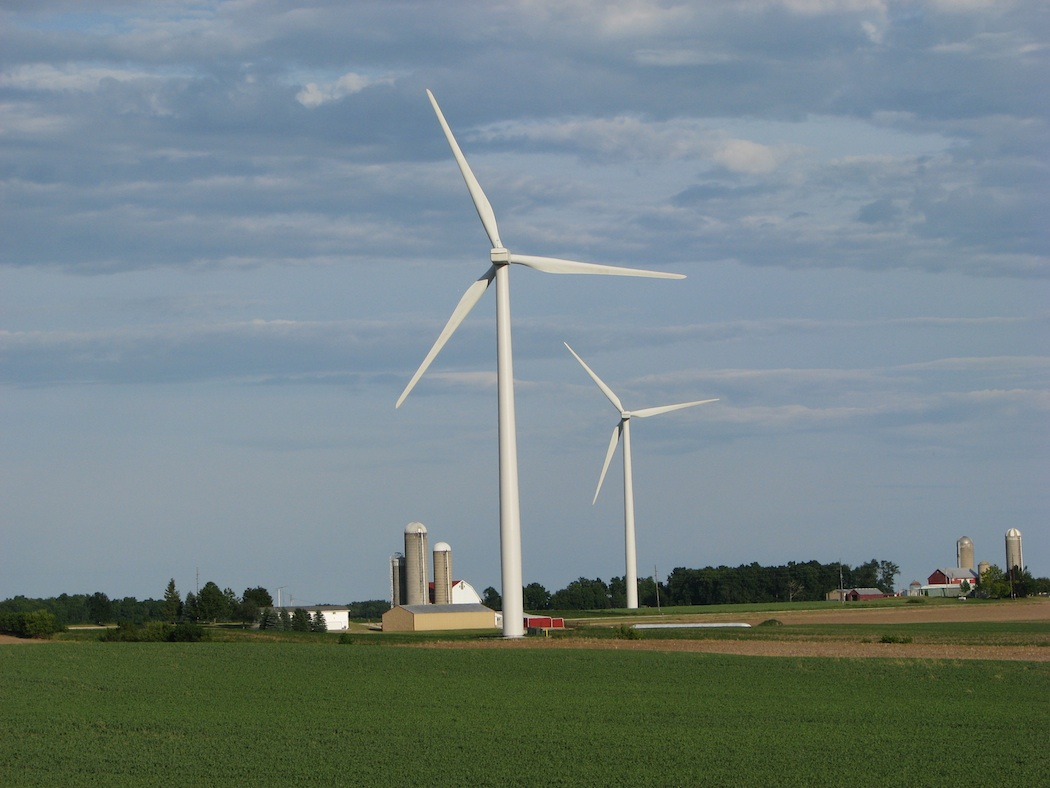
\includegraphics[height=2.5in]{files/21206}
            \caption{Wind turbines at the Forward Wind Energy Center in Fond du Lac and Dodge Counties, Wisconsin. (Photo by Ruth Baranowski / NREL)}\label{fig:21206}
          \end{subfigure}%
          \begin{subfigure}[b]{.5\linewidth}
            \centering
            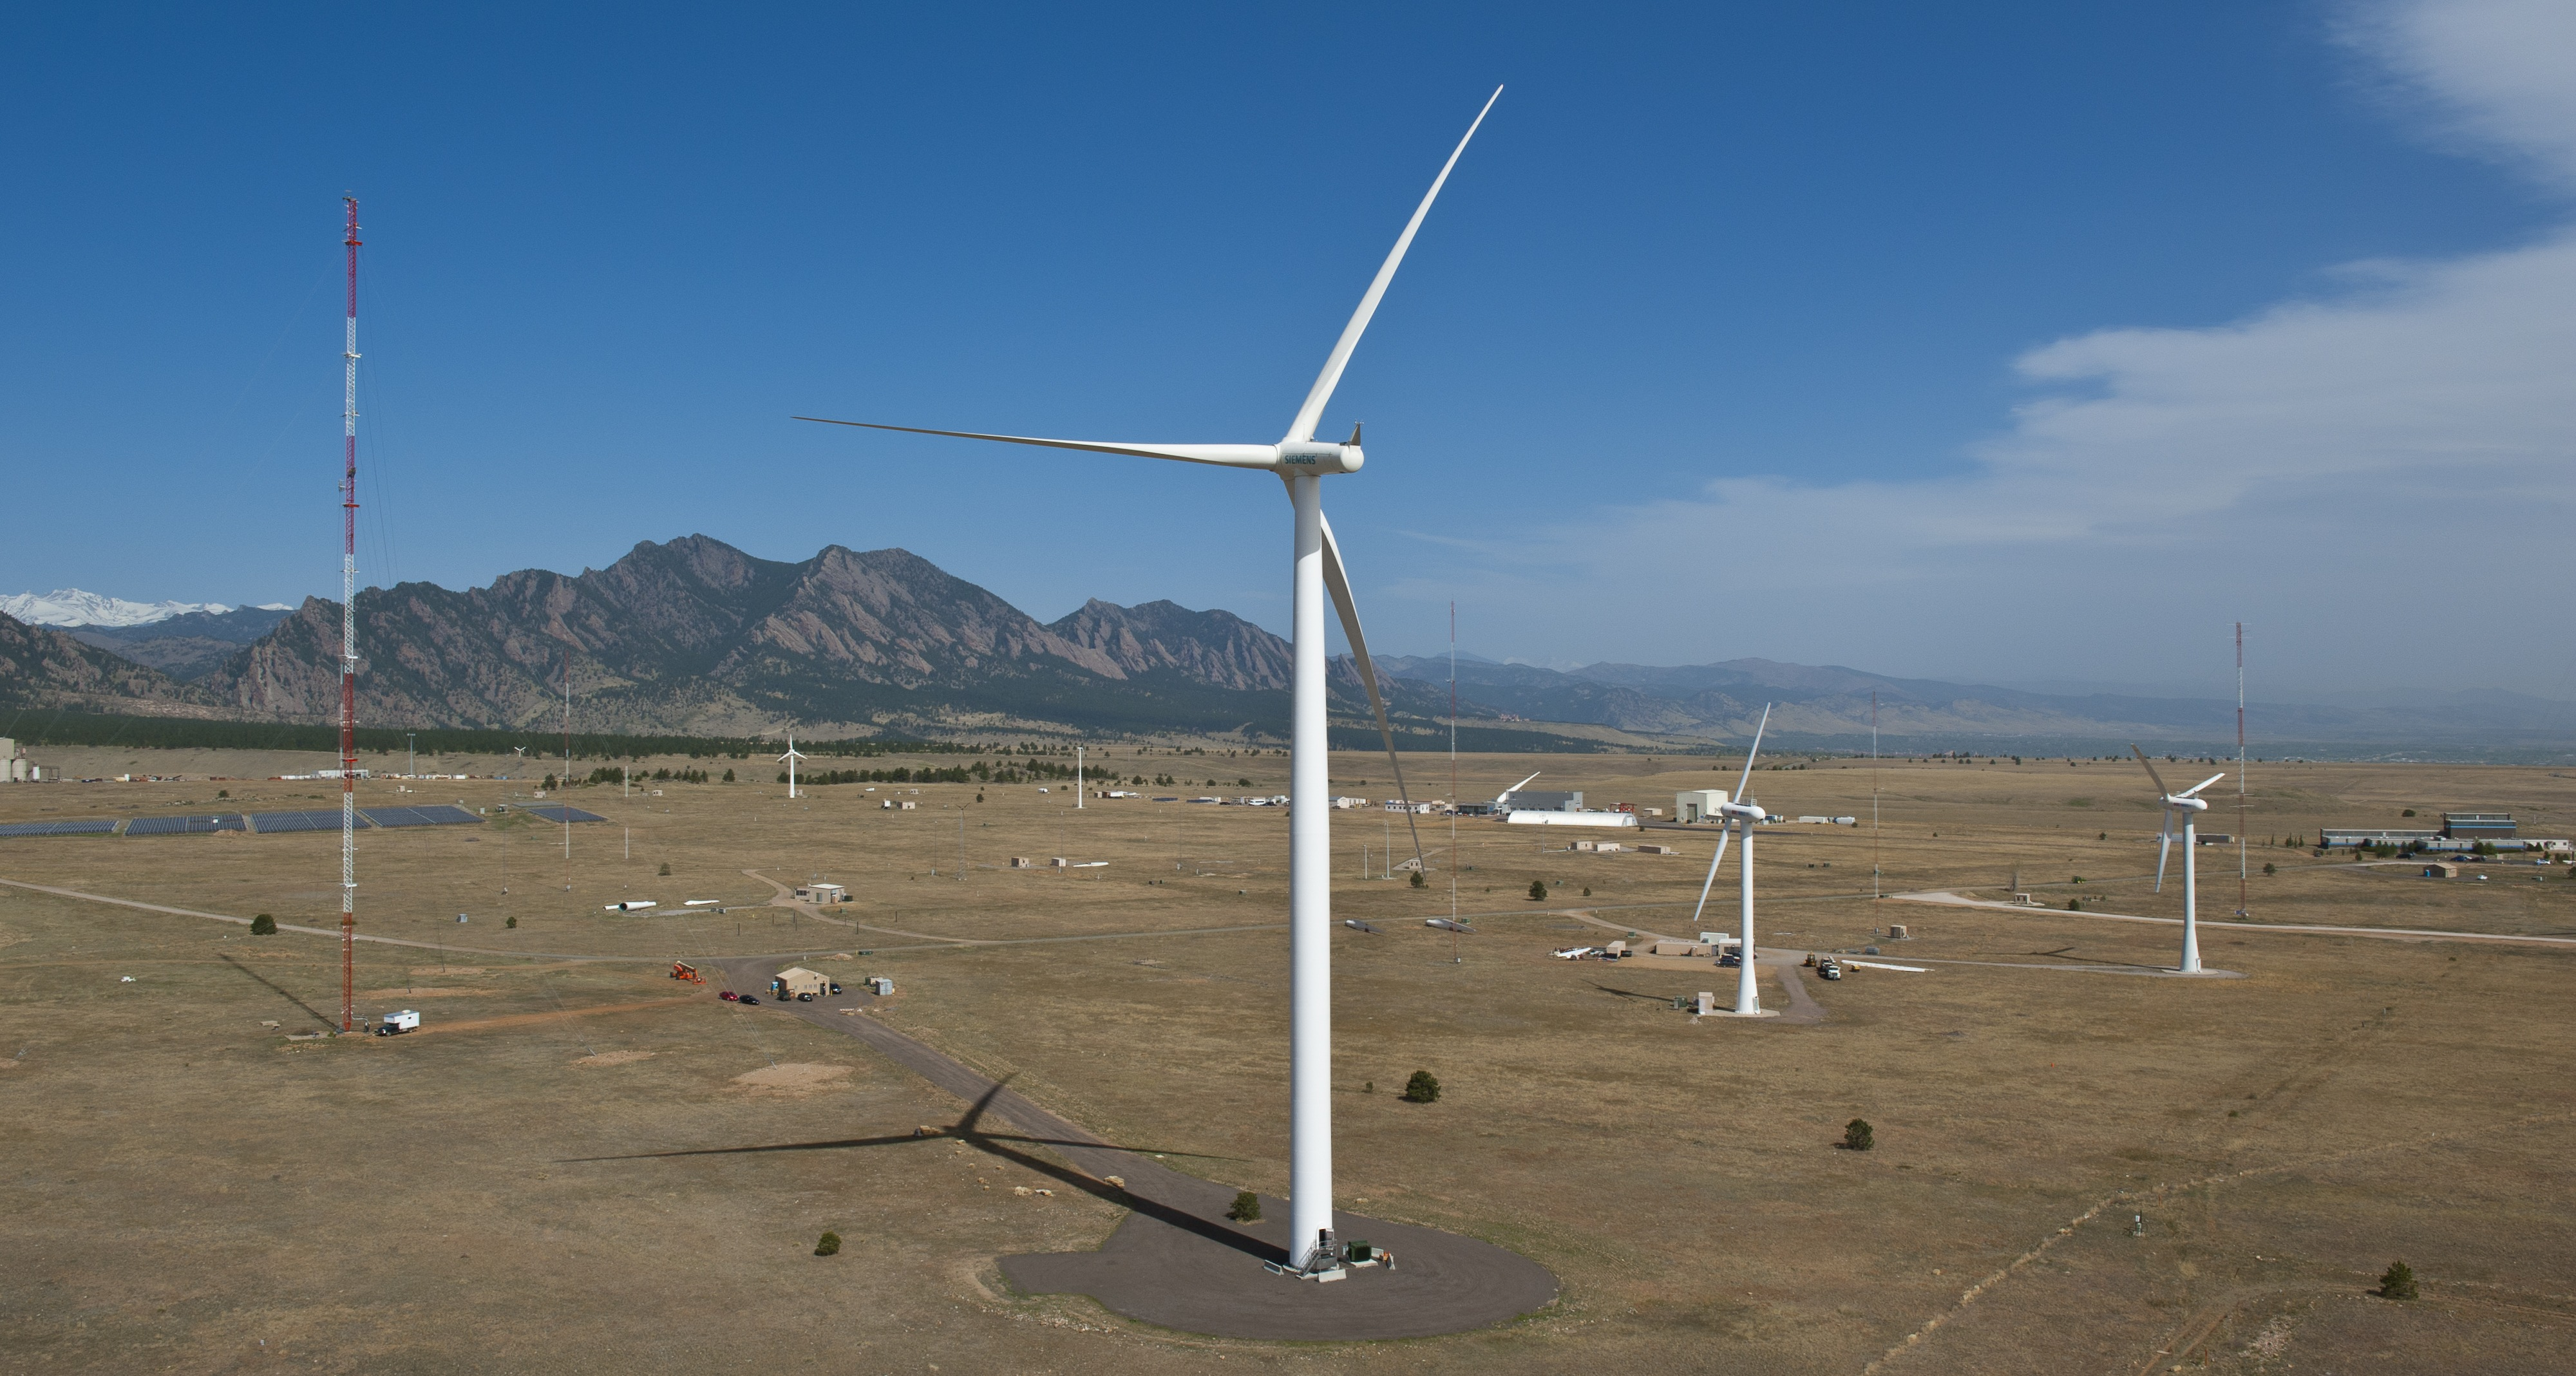
\includegraphics[height=2.5in]{files/20018}
            \caption{Aerial view of the National Wind Technology Center. (Photo by Dennis Schroeder / NREL)}\label{fig:20018}
          \end{subfigure}
          \caption{Images}\label{fig:NRELimages}
\end{figure}
\end{lstlisting}

Note that the \texttt{subfig} and \texttt{subfigure} packages are deprecated. The \texttt{subcaption} package appears to be the most frequently maintained package at this time, and contains the same functionality as the \texttt{subfig} and \texttt{subfigure} packages.

\begin{figure*}
          \begin{subfigure}[t]{.55\linewidth}
            \centering
            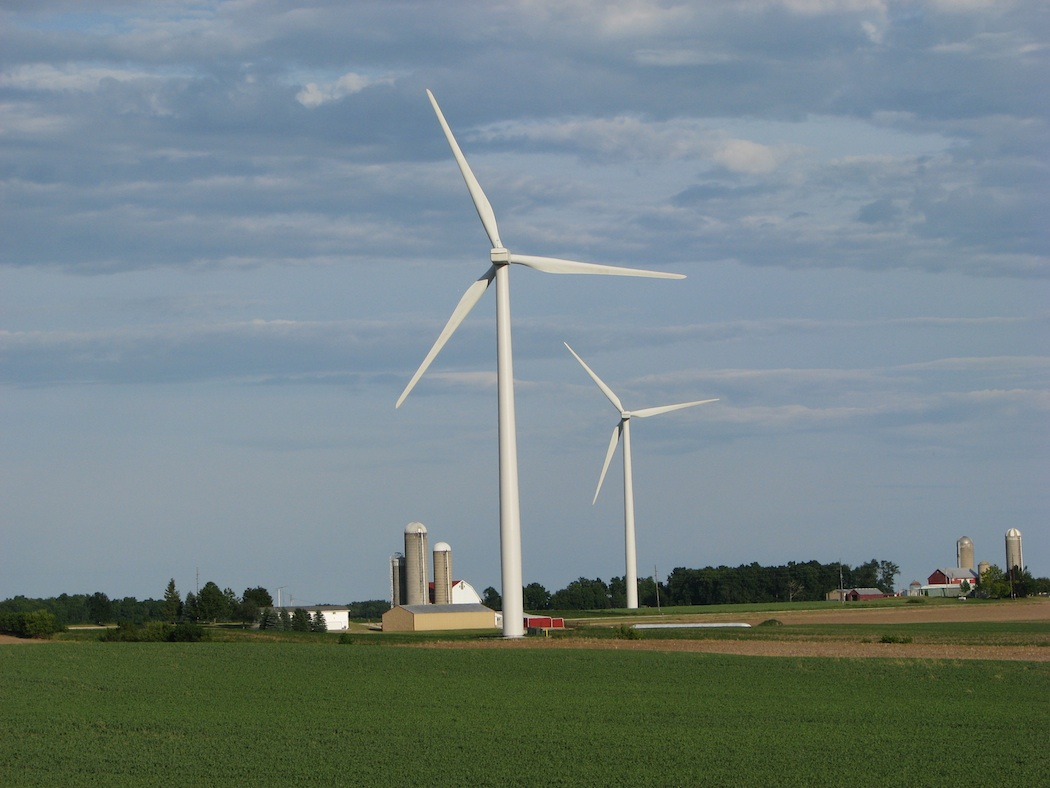
\includegraphics[height=2.5in]{files/21206}
            \caption{Wind turbines at the Forward Wind Energy Center in Fond du Lac and Dodge Counties, Wisconsin. (Photo by Ruth Baranowski / NREL)}\label{fig:21206}
          \end{subfigure}%
          \begin{subfigure}[t]{.55\linewidth}
            \centering
            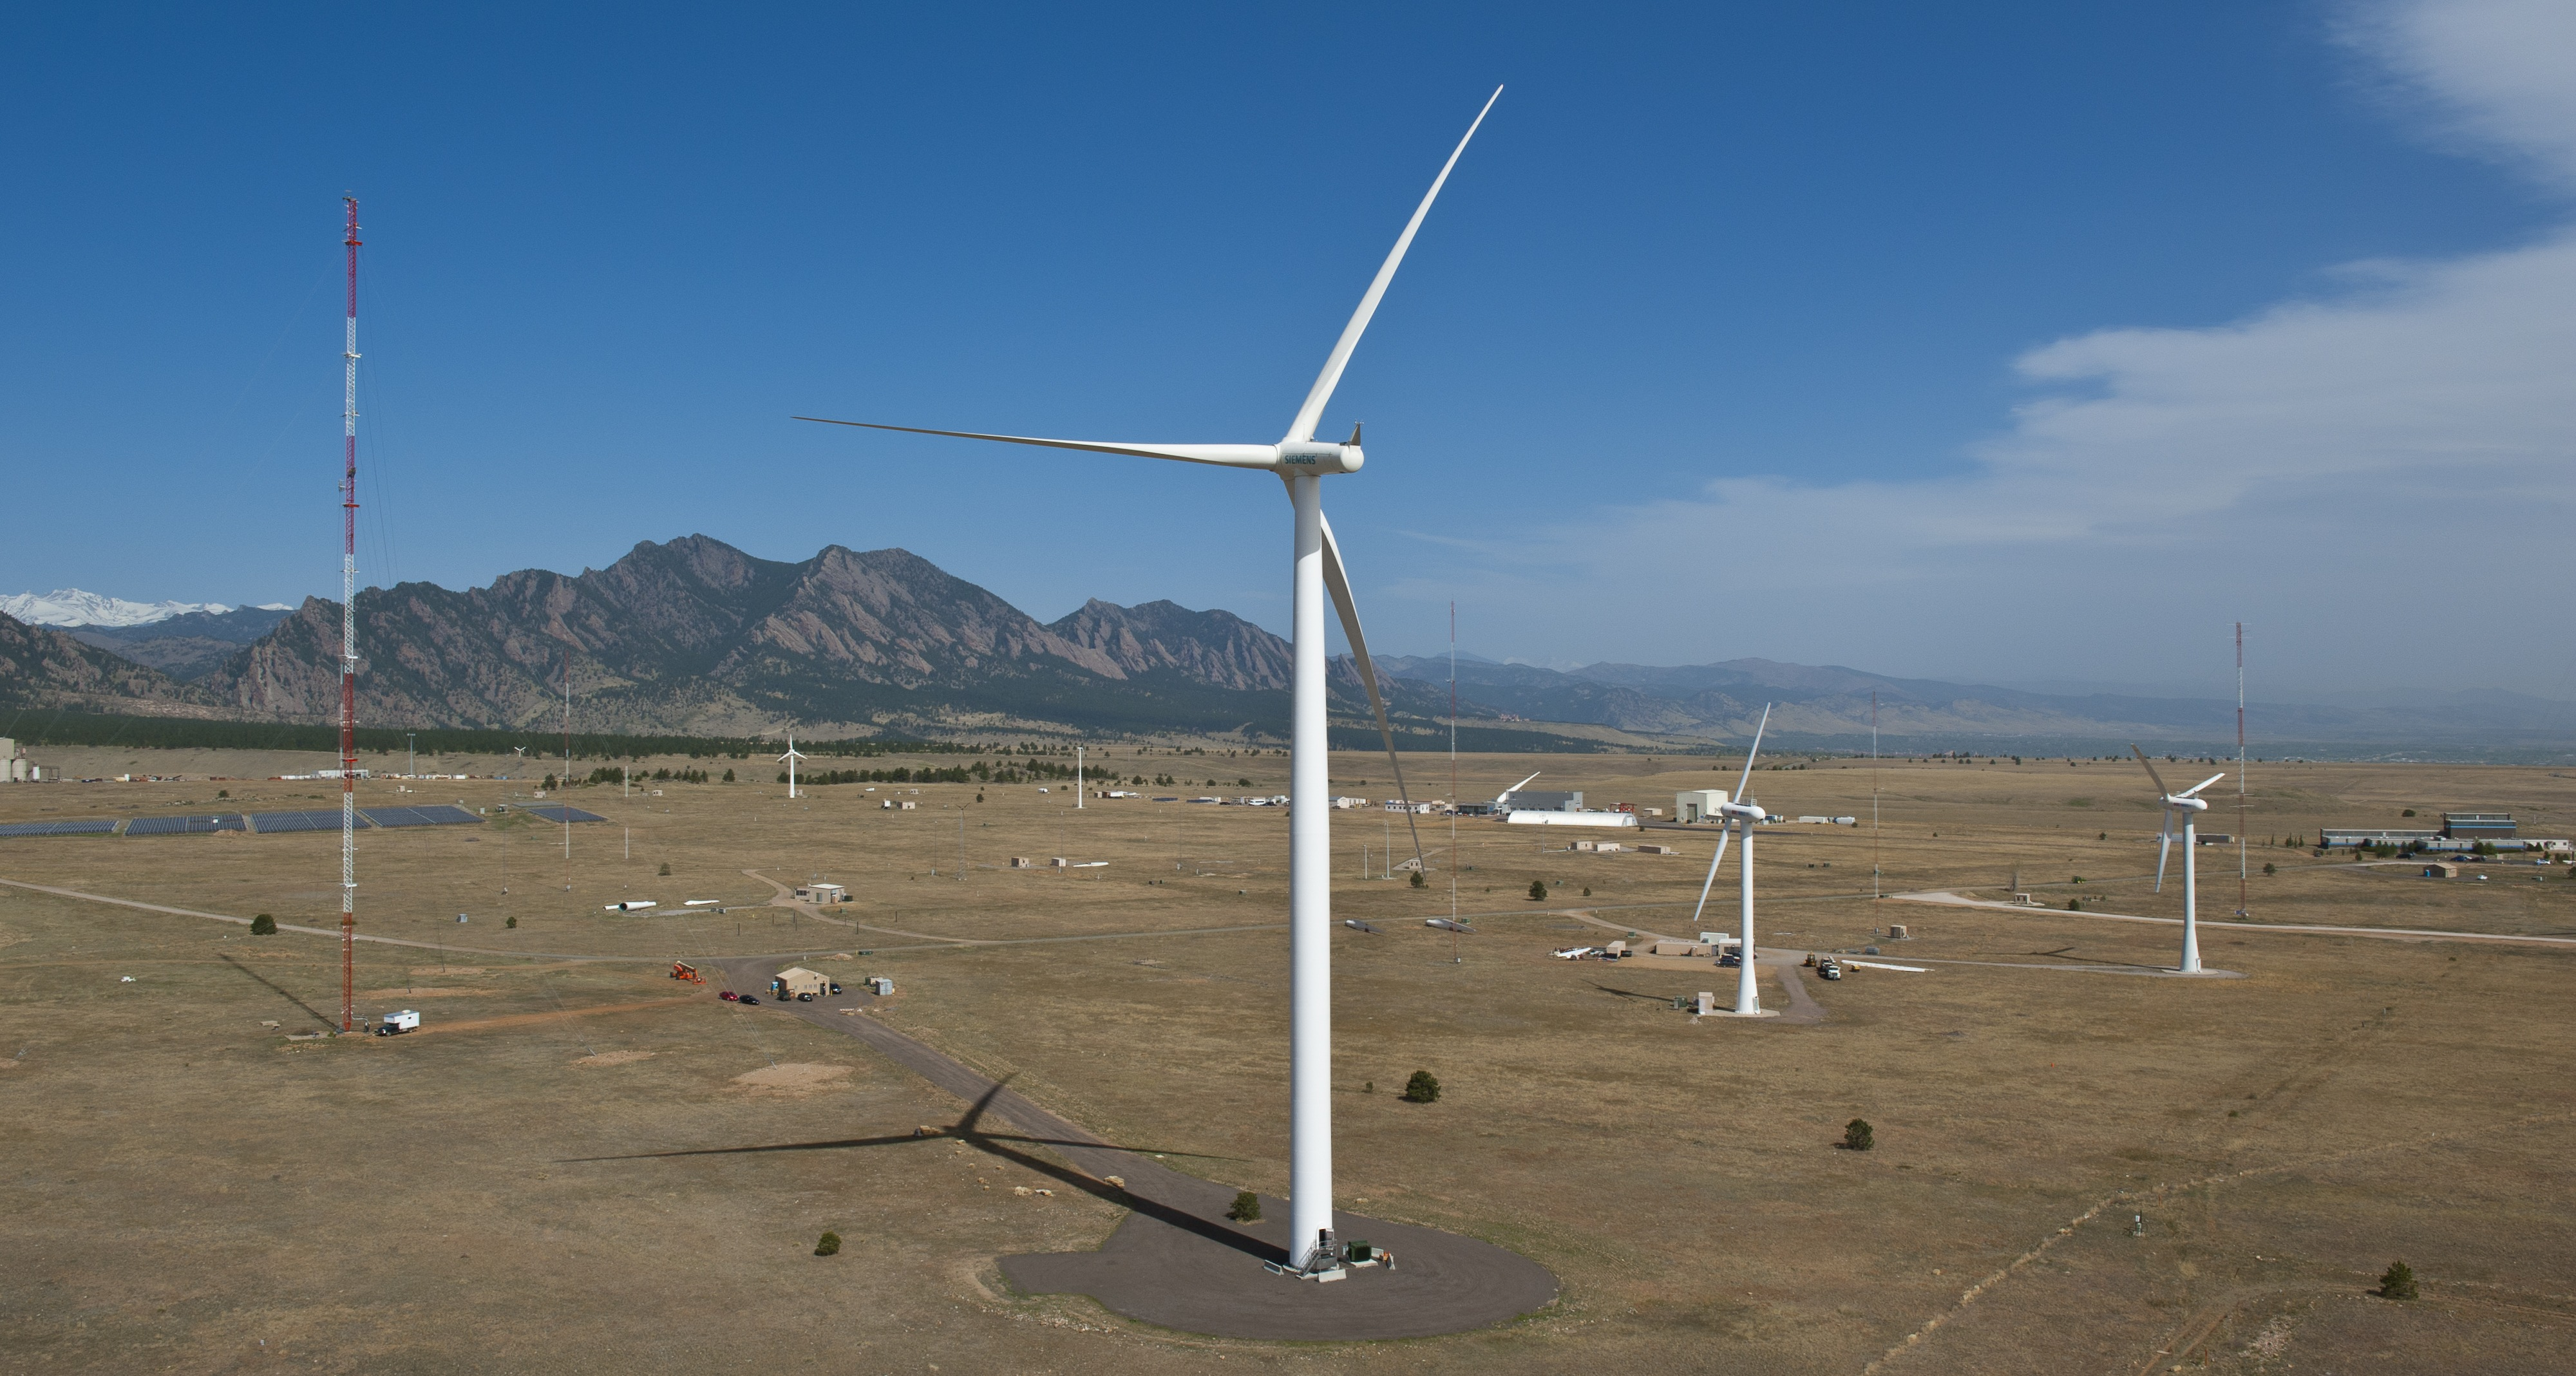
\includegraphics[height=2.5in]{files/20018}
            \caption{Aerial view of the National Wind Technology Center. (Photo by Dennis Schroeder / NREL)}\label{fig:20018}
          \end{subfigure}
          \caption{Images}\label{fig:NRELimages}
\end{figure*}

\subsubsection{Citations}
\label{Sec:Bib}
Use \texttt{bibtex} to organize references and store them in a single file (e.g. \verb+/Documents/bibliography/bibliography.bib+). The bibliography will then contain entries with `keys' for each source, like \texttt{Lamport\_1986\_a}. 

Authors can then insert citations to this key throughout their document, using different styles of citation. Citations are generated using the \texttt{biblatex} package, which also formats references in the correct style.  Ways to generate citations are described in the \texttt{biblatex} documentation, and include:
\begin{itemize}
\item \verb+\cite{Lamport_1986_a}+ prints \cite{Lamport_1986_a}.
\item \verb+\citep{Lamport_1986_a}+ prints \citep{Lamport_1986_a}.
\item \verb+\citet{Lamport_1986_a}+ prints \citet{Lamport_1986_a}.
\end{itemize}

To cite URLs, use the 'misc' style. For example, the bibtex entry for \href{http://tex.stackexchange.com}{http://tex.stackexchange.com}\ \cite{texstackexchange} looks like this:

\begin{lstlisting}
@misc{texstackexchange,
	Author = {Anon.},
	Howpublished = {Accessed July 21, 2014: \url{http://tex.stackexchange.com}},
	Title = {\TeX -- LaTeX Stack Exchange},
	Year = {2014}}
\end{lstlisting}

This format will allow you to include the date on which a URL was accessed.

The citations should work with journal articles \citep{Clifton_2013_a}, books \citep{Knuth_1984_a, Lamport_1986_a, chicago}, technical reports \citep{TechReportTest}, and URLs \citep{texstackexchange}. Any unknown publication types will be formatted using the `misc' type.

\subsubsection{Including computer code}
The \texttt{listings} package has been loaded. Note: this does not work if the `Draft' document option is used.

To change the syntax highlighting use \verb+\lstset{language=[dialect]language, columns=fullflexible, keepspaces=true}+ before each listing where the language changes. For more details see the \texttt{lstlisting} documentation.

\subsubsection{Bibliographies}
This document class uses "Chicago A" style-references produced using Biblatex. The reference style can be changed in the \emph{CorporateArticle.cls} file.

To include a bibliography in the document give the bibliography file location in the preamble and insert the bibliography at the appropriate location:

\begin{lstlisting}
% give the bibliography file location
\bibliography{files/bibliography.bib}
...
\begin{document}
...
% insert the bibliography into the document
\cleardoublepage
\label{sec:Bib}
\printbibliography
...
\end{document}
\end{lstlisting}

An example bibliography is included in this document on page \pageref{sec:Bib}.

\subsubsection{Footnotes}
Footnotes can be inserted using the \verb+\footnote{}+ command\footnote{like this}. Footnotes are numbered in the main matter\footnote{and like this as well}, and use daggers, etc instead of numers in the appendices.

\subsection{Creating a file structure}
\label{sec:FileStructure}
Your main file should be called \emph{main.tex}. This helps editors and coauthors identify where to start. Then, use \texttt{input} to import other files into your main file at compilation.

For example, each of the chapters in this report is in separate files, called \emph{WhatIsLatex} (Chapter 1), \emph{LatexForDocs} (Chapter 2), and so-on. In the example available on Github, they are stored in the \emph{files} directory. \emph{main.tex} then looks like this:

\begin{lstlisting}
...
\begin{document}
% content
\chapter{What is LaTeX?}
LaTeX is a mark-up language that describes how a document should be prepared. Three things are needed to make a LaTeX document:
\begin{enumerate}
\item A source document, usually with extension \emph{.tex}
\item Some packages and classes that help turn what's in the source document into something helpful
\item A compiler, also referred to as a working LaTeX installation.
\end{enumerate}

At first glance the source document looks like a programming language, and that's because it is: LaTeX is not WYSIWYG, like many of the document preparation tools in common use today. A good analogy is html.

\section{Printed Resources}


\section{Online Resources}
The wikibook at \href{http://en.wikibooks.org/wiki/LaTeX}{http://en.wikibooks.org/wiki/LaTeX} is an excellent resource. There are also several internet forums such as \href{tex.stackexchange.com}{tex.stackexchange.com} that may be useful.

Documentation for the packages used in the nrel.cls file (Section \ref{sec:nrelcls}) can be found at \href{ctan.org}{ctan.org}.

\section{Using LaTeX to Make Corporate Documents }
A series of LaTeX class files called \emph{Corporate...cls} have been written to implement common formatting requirements in LaTeX.

\subsection{Corporate class files}\label{sec:Corporatecls}
Class files control the formatting and presentation of documents. The class files currently available include:
\begin{description}
\item[CorporateReport.cls]{compiles the document using the LaTeX \emph{report} class, with corporate formatting. This is intended for longer documents and allows the use of chapters.}
\item[CorporateArticle.cls] compiles the document using the LaTeX \emph{article} class, with corporate formatting. This is intended for shorter documents such as journal articles. This class does not support the use of chapters.
\item[CorporateResources.tex] contains the common packages and formatting descriptions that are implemented by the \emph{CorporateReport.cls} and \emph{CorporateArticle.cls} classes.
\end{description}

As with normal classes, options are passed to the class in the \verb+\documentclass+ line:

\begin{lstlisting}
\documentclass[option1,...,optionn]{CorporateArticle}
\end{lstlisting}

Options specific to \emph{Corporate*.cls} include:
\begin{description}
\item[draft]{add a `draft' watermark to all pages.}
\end{description}

The \emph{Corporate....cls} files call a variety of other packages. Packages are codes that modify the appearance or behaviour of LaTeX to achieve something. Table \ref{Tab:Packages} lists the packages that are explicitly called by \emph{Corporate*.cls} or \emph{CorporateResources.tex} in the order they are called in. These packages often call other packages, so this is not an exhaustive list.

\begin{table*}[!h]
\centering
\caption[Packages loaded by the Corporate classes]{Packages loaded by the Corporate classes.}
\label{Tab:Packages}
\begin{tabular*}{\textwidth}{llp{0.6\textwidth}}
\toprule
Package & Options & Functionality\\
\midrule
%accessibility & tagged & generates the document structure and tagging \\
amsfonts, amssymb & & supplies AMS fonts, which are useful for mathematics \\
babel & english & activates language-appropriate hyphenation rules\\
booktabs & & improves the formatting of tables \\
caption & & required to generate captions for floats\\
fontenc & T1 & enables direct typing of international characters \\
geometry & & sets page size and margins \\
graphicx & & graphics handling, including \emph{.eps} figures \\
hyphenat & & improves spacing and breaking of hyphenated words \\
listings & & enables the inclusion of high-quality computer code listings\\
nag & & checks that packages are up to date and looks for bad habits in LaTeX code. \\
parskip & & required for better spacing\\
pdfcomment & & required for tool-tips. Also calls the \texttt{hyperref} package  \\
setspace & & required for better spacing\\
subcaption & & provides the \texttt{subfigure} environment to produce sub figures \\
tocloft & & improved table of contents and list of figures/tables in memoir documents\\
tocbibind & nottoc, notlot, notlof & Add bibliography/index/contents to Table of Contents in memoir documents\\
todonotes & & inline and margin to-do notes \\
xcolor & & Driver-independent color extensions for LaTeX and pdfLaTeX\\
\bottomrule
\end{tabular*}
\end{table*}

It should be noted that the `english` option to Babel really means \emph{American} English.

\subsubsection{Starting new documents}
\begin{enumerate}
\item Go to \href{https://github.com/xx}{https://github.com/xx} and download the latest version of the repository as a .zip file from the icon on the lower right hand side of the page.
\item ...
\item Modify \emph{main.tex} as required.
\end{enumerate}

\subsection{Creating Content}
\subsubsection{Front, main, and back matter}
The convention in this corporate class is to have Roman numerals in the front matter, and then arabic numerals in the main matter of the document (after the tables of contents, figures and tables). Tables and figures in the front matter are also numbered differently (Table A, B, C, ...) than in the main matter (Table 1, 2, 3, ...).

This change in page and float numbering is implemented using the \verb+\frontmatter+, \verb+\mainmatter+, and \verb+\backmatter+ commands at the start of these sections of the document:

\begin{lstlisting}
\begin{document}

\maketitle
\frontmatter
...
\tableofcontents
\clearpage
\listoffigures
\listoftables
\mainmatter
...
\backmatter
\end{document}
\end{lstlisting}

Page numbering in the front matter (i.e. the Abstract, Summary, and Foreword chapters or sections) starts at page 3 to allow for cover pages.

If you don't use the \verb+\frontmatter+ commands, you may need to increment the page counter manually. To increment the counter $n$ pages, use \verb+\setcounter{page}{n}+ after \verb+\begin{document}+.

\subsubsection{Cross references}
Use labels and references to refer back and forth to figures, equations, tables and sections. 

For example, an equation can be added using the following text:

\begin{lstlisting}
\begin{equation}
y = mx+c
\label{eqn:line}
\end{equation}
\end{lstlisting}

This gives the following:
\begin{equation}
y = mx+c
\label{eqn:line}
\end{equation}

And using the text \verb+Eqn. \ref{eqn:line}+ provides a cross reference to Eqn. \ref{eqn:line}.

\subsubsection{Floats}
Floats are images, tables or other pieces of the document that are free to move to the best place in the document for them. The two most common floats are the tabular environment (for tables) and the figure environment for figures.

\paragraph{Tables}
Use the \texttt{tabular} environment to produce basic tables. Table~\ref{tab:widgets} is produced using this code: 

\begin{lstlisting}
\begin{table}[!h]
\centering
\caption{An example table.}\label{tab:widgets}
\begin{tabular}{lr}
Item & Quantity \\
\hline
Widgets & 42 \\
Gadgets & 13
\end{tabular}
\end{table}
\end{lstlisting}

\begin{table}[!h]
\centering
\caption{An example table.}\label{tab:widgets}
\begin{tabular}{lr}
Item & Quantity \\
\hline
Widgets & 42 \\
Gadgets & 13
\end{tabular}
\end{table}

If all of the delimiters (\&) are included in each row, the table will be complete and will produce a better PDF.

\paragraph{Figures}
To include a figure in a document, use the \texttt{figure} environment and the \texttt{includegraphics} command.

\begin{lstlisting}
\begin{figure}
\includegraphics[width=\textwidth]{figure's-file-name}
\caption{Caption goes here.}\label{fig:figuresLabel}
\end{figure}
\end{lstlisting}

\paragraph{Subfigures}

Subfigures are implemented using the \texttt{subcaption} package. The example below generates Figure \ref{fig:NRELimages}.

\begin{lstlisting}
\begin{figure}
          \begin{subfigure}[b]{.5\linewidth}
            \centering
            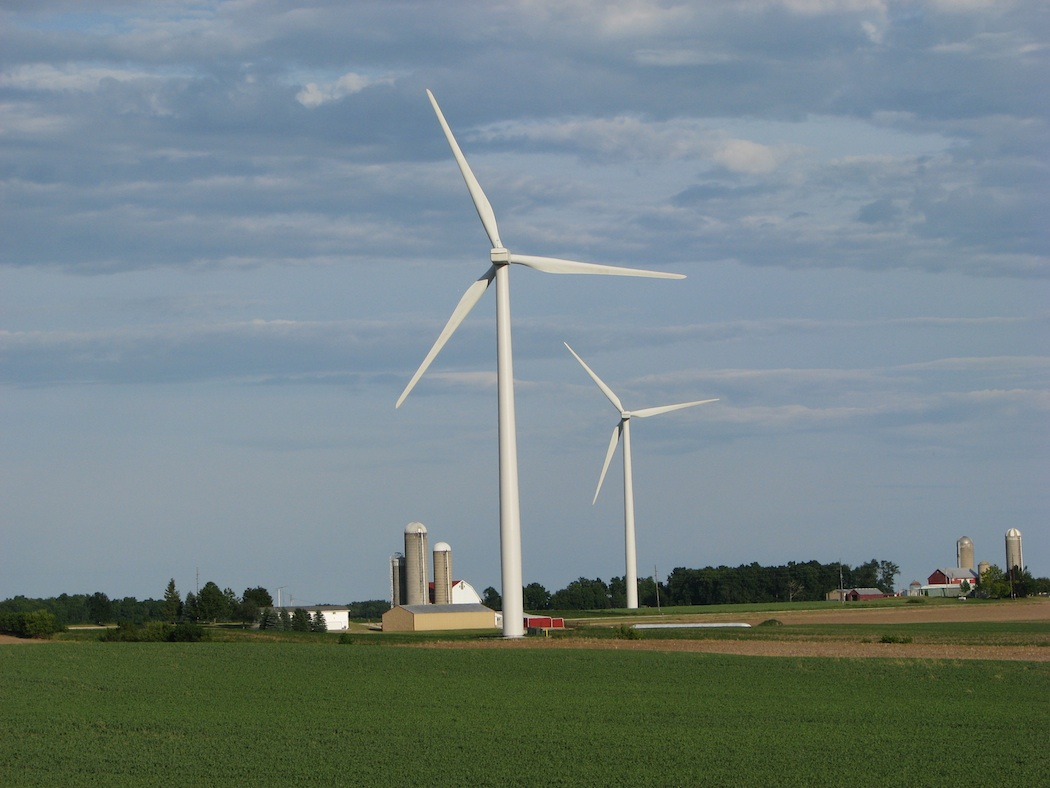
\includegraphics[height=2.5in]{files/21206}
            \caption{Wind turbines at the Forward Wind Energy Center in Fond du Lac and Dodge Counties, Wisconsin. (Photo by Ruth Baranowski / NREL)}\label{fig:21206}
          \end{subfigure}%
          \begin{subfigure}[b]{.5\linewidth}
            \centering
            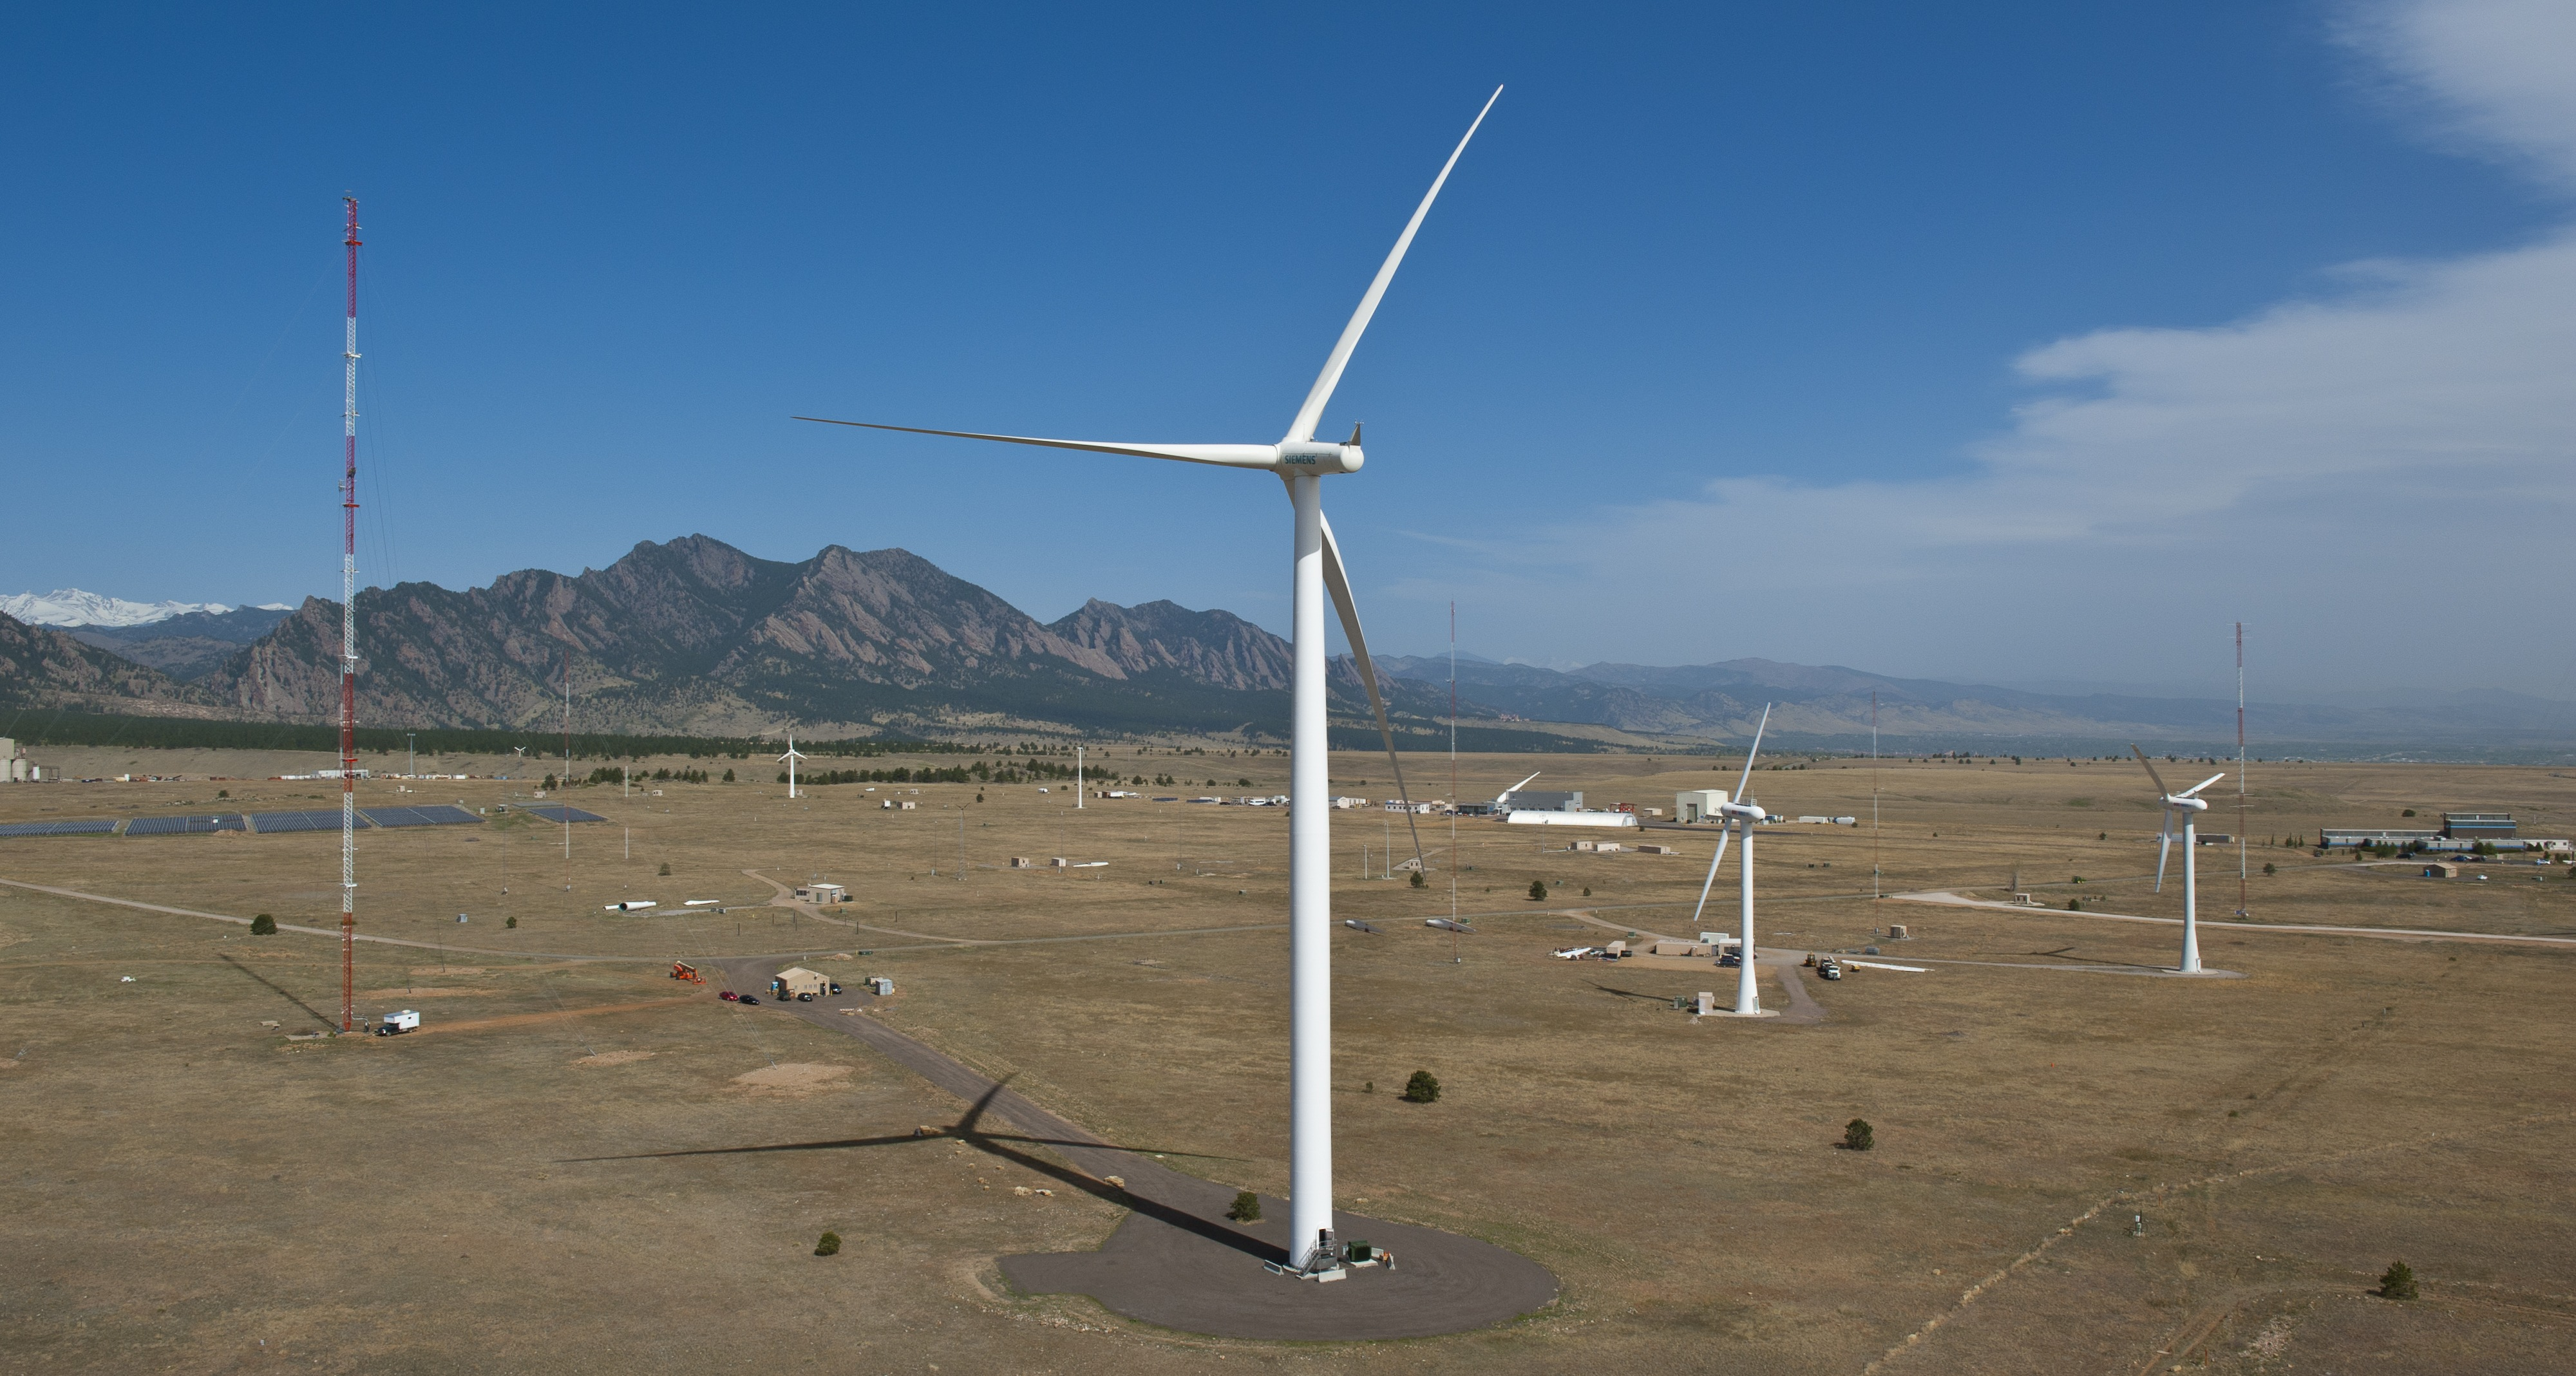
\includegraphics[height=2.5in]{files/20018}
            \caption{Aerial view of the National Wind Technology Center. (Photo by Dennis Schroeder / NREL)}\label{fig:20018}
          \end{subfigure}
          \caption{Images}\label{fig:NRELimages}
\end{figure}
\end{lstlisting}

Note that the \texttt{subfig} and \texttt{subfigure} packages are deprecated. The \texttt{subcaption} package appears to be the most frequently maintained package at this time, and contains the same functionality as the \texttt{subfig} and \texttt{subfigure} packages.

\begin{figure*}
          \begin{subfigure}[t]{.55\linewidth}
            \centering
            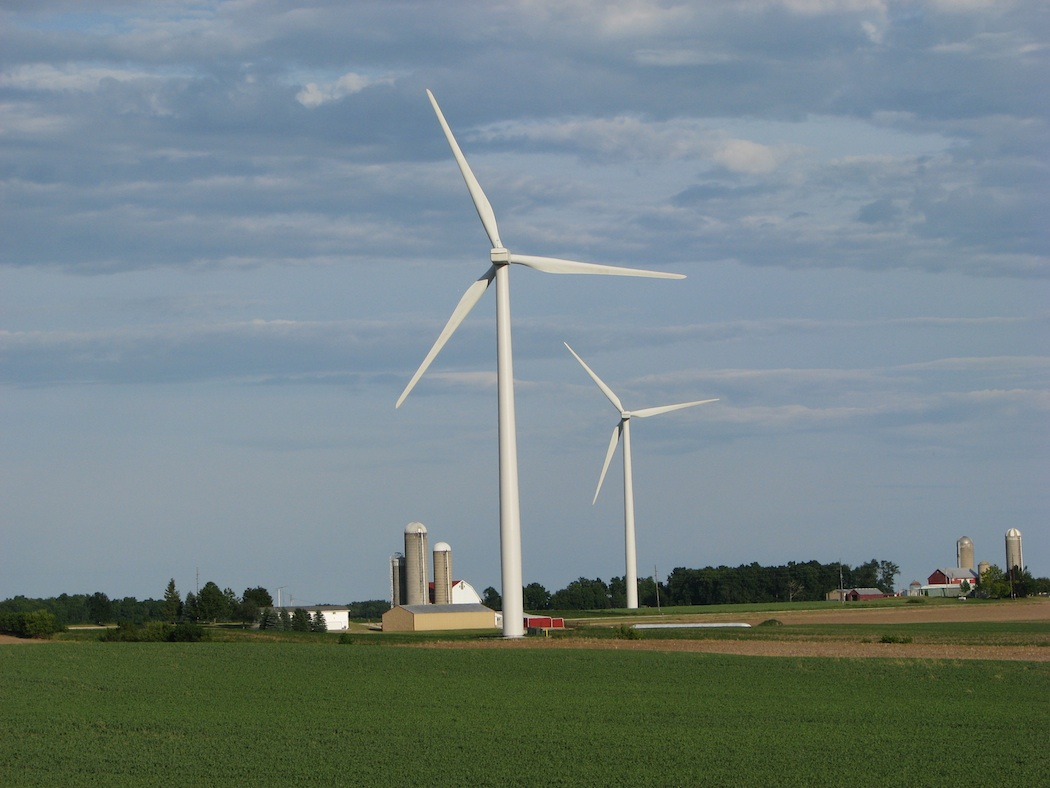
\includegraphics[height=2.5in]{files/21206}
            \caption{Wind turbines at the Forward Wind Energy Center in Fond du Lac and Dodge Counties, Wisconsin. (Photo by Ruth Baranowski / NREL)}\label{fig:21206}
          \end{subfigure}%
          \begin{subfigure}[t]{.55\linewidth}
            \centering
            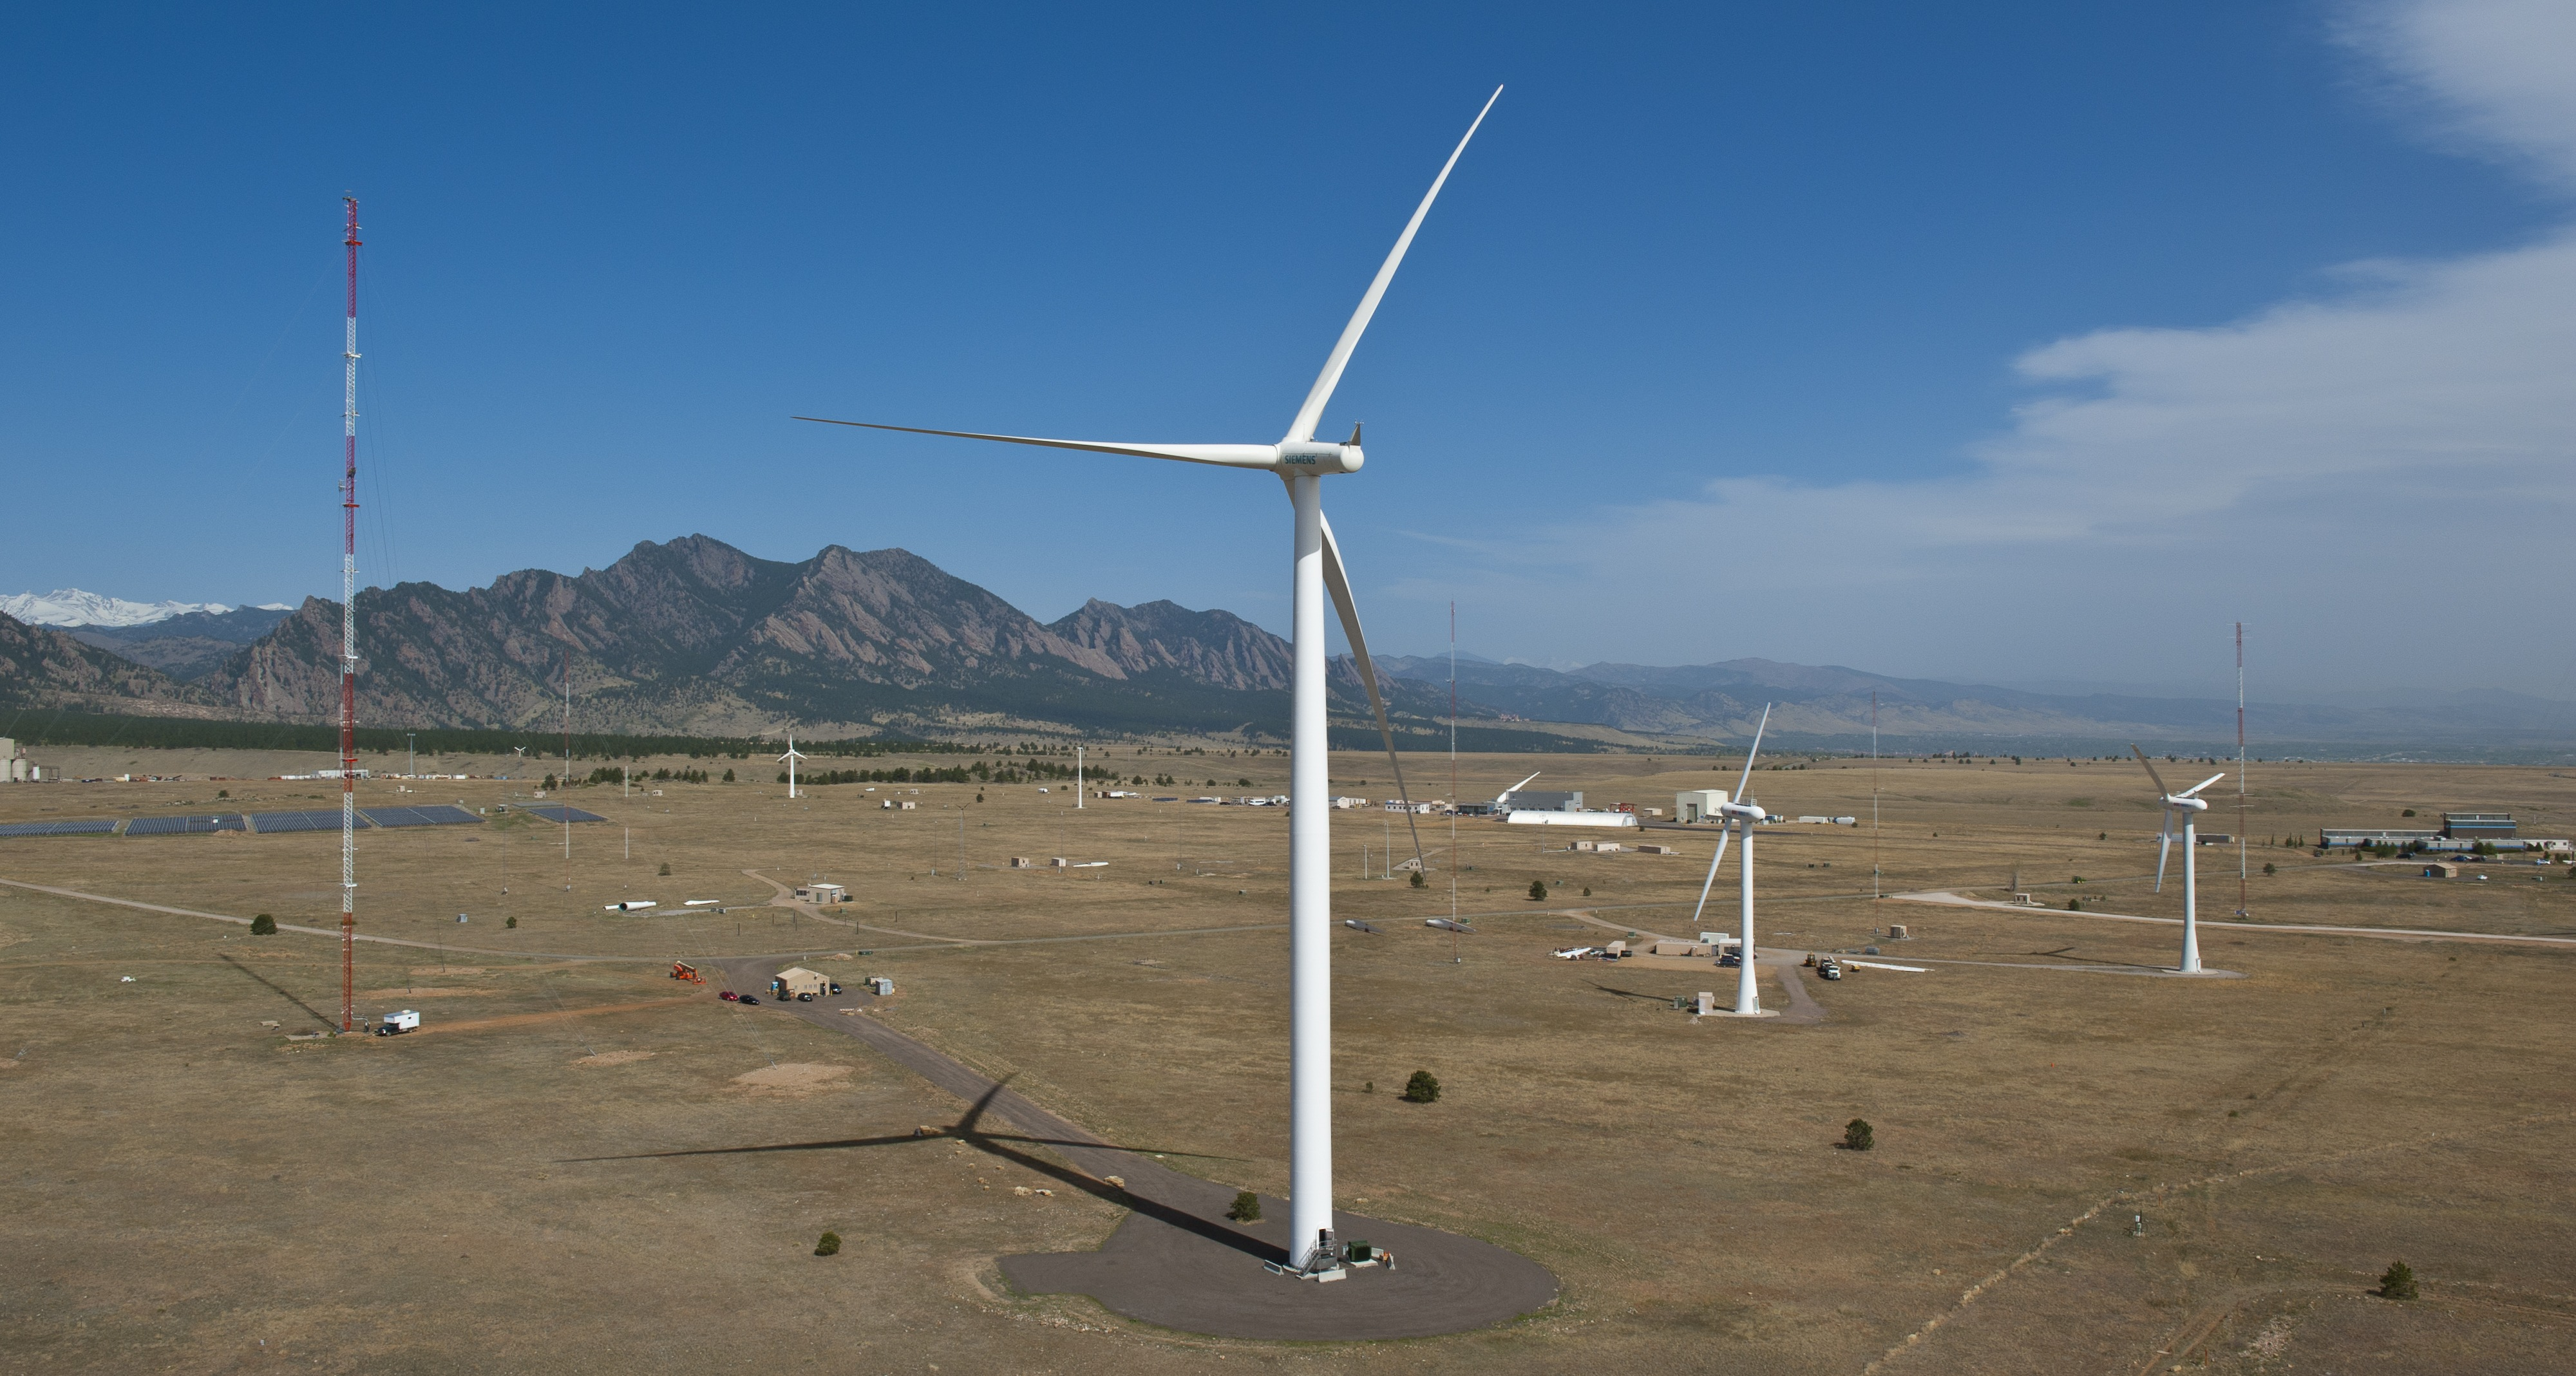
\includegraphics[height=2.5in]{files/20018}
            \caption{Aerial view of the National Wind Technology Center. (Photo by Dennis Schroeder / NREL)}\label{fig:20018}
          \end{subfigure}
          \caption{Images}\label{fig:NRELimages}
\end{figure*}

\subsubsection{Citations}
\label{Sec:Bib}
Use \texttt{bibtex} to organize references and store them in a single file (e.g. \verb+/Documents/bibliography/bibliography.bib+). The bibliography will then contain entries with `keys' for each source, like \texttt{Lamport\_1986\_a}. 

Authors can then insert citations to this key throughout their document, using different styles of citation. Citations are generated using the \texttt{biblatex} package, which also formats references in the correct style.  Ways to generate citations are described in the \texttt{biblatex} documentation, and include:
\begin{itemize}
\item \verb+\cite{Lamport_1986_a}+ prints \cite{Lamport_1986_a}.
\item \verb+\citep{Lamport_1986_a}+ prints \citep{Lamport_1986_a}.
\item \verb+\citet{Lamport_1986_a}+ prints \citet{Lamport_1986_a}.
\end{itemize}

To cite URLs, use the 'misc' style. For example, the bibtex entry for \href{http://tex.stackexchange.com}{http://tex.stackexchange.com}\ \cite{texstackexchange} looks like this:

\begin{lstlisting}
@misc{texstackexchange,
	Author = {Anon.},
	Howpublished = {Accessed July 21, 2014: \url{http://tex.stackexchange.com}},
	Title = {\TeX -- LaTeX Stack Exchange},
	Year = {2014}}
\end{lstlisting}

This format will allow you to include the date on which a URL was accessed.

The citations should work with journal articles \citep{Clifton_2013_a}, books \citep{Knuth_1984_a, Lamport_1986_a, chicago}, technical reports \citep{TechReportTest}, and URLs \citep{texstackexchange}. Any unknown publication types will be formatted using the `misc' type.

\subsubsection{Including computer code}
The \texttt{listings} package has been loaded. Note: this does not work if the `Draft' document option is used.

To change the syntax highlighting use \verb+\lstset{language=[dialect]language, columns=fullflexible, keepspaces=true}+ before each listing where the language changes. For more details see the \texttt{lstlisting} documentation.

\subsubsection{Bibliographies}
This document class uses "Chicago A" style-references produced using Biblatex. The reference style can be changed in the \emph{CorporateArticle.cls} file.

To include a bibliography in the document give the bibliography file location in the preamble and insert the bibliography at the appropriate location:

\begin{lstlisting}
% give the bibliography file location
\bibliography{files/bibliography.bib}
...
\begin{document}
...
% insert the bibliography into the document
\cleardoublepage
\label{sec:Bib}
\printbibliography
...
\end{document}
\end{lstlisting}

An example bibliography is included in this document on page \pageref{sec:Bib}.

\subsubsection{Footnotes}
Footnotes can be inserted using the \verb+\footnote{}+ command\footnote{like this}. Footnotes are numbered in the main matter\footnote{and like this as well}, and use daggers, etc instead of numers in the appendices.

\subsection{Creating a file structure}
\label{sec:FileStructure}
Your main file should be called \emph{main.tex}. This helps editors and coauthors identify where to start. Then, use \texttt{input} to import other files into your main file at compilation.

For example, each of the chapters in this report is in separate files, called \emph{WhatIsLatex} (Chapter 1), \emph{LatexForDocs} (Chapter 2), and so-on. In the example available on Github, they are stored in the \emph{files} directory. \emph{main.tex} then looks like this:

\begin{lstlisting}
...
\begin{document}
% content
\chapter{What is LaTeX?}
LaTeX is a mark-up language that describes how a document should be prepared. Three things are needed to make a LaTeX document:
\begin{enumerate}
\item A source document, usually with extension \emph{.tex}
\item Some packages and classes that help turn what's in the source document into something helpful
\item A compiler, also referred to as a working LaTeX installation.
\end{enumerate}

At first glance the source document looks like a programming language, and that's because it is: LaTeX is not WYSIWYG, like many of the document preparation tools in common use today. A good analogy is html.

\section{Printed Resources}


\section{Online Resources}
The wikibook at \href{http://en.wikibooks.org/wiki/LaTeX}{http://en.wikibooks.org/wiki/LaTeX} is an excellent resource. There are also several internet forums such as \href{tex.stackexchange.com}{tex.stackexchange.com} that may be useful.

Documentation for the packages used in the nrel.cls file (Section \ref{sec:nrelcls}) can be found at \href{ctan.org}{ctan.org}.

\section{Using LaTeX to Make Corporate Documents }
A series of LaTeX class files called \emph{Corporate...cls} have been written to implement common formatting requirements in LaTeX.

\subsection{Corporate class files}\label{sec:Corporatecls}
Class files control the formatting and presentation of documents. The class files currently available include:
\begin{description}
\item[CorporateReport.cls]{compiles the document using the LaTeX \emph{report} class, with corporate formatting. This is intended for longer documents and allows the use of chapters.}
\item[CorporateArticle.cls] compiles the document using the LaTeX \emph{article} class, with corporate formatting. This is intended for shorter documents such as journal articles. This class does not support the use of chapters.
\item[CorporateResources.tex] contains the common packages and formatting descriptions that are implemented by the \emph{CorporateReport.cls} and \emph{CorporateArticle.cls} classes.
\end{description}

As with normal classes, options are passed to the class in the \verb+\documentclass+ line:

\begin{lstlisting}
\documentclass[option1,...,optionn]{CorporateArticle}
\end{lstlisting}

Options specific to \emph{Corporate*.cls} include:
\begin{description}
\item[draft]{add a `draft' watermark to all pages.}
\end{description}

The \emph{Corporate....cls} files call a variety of other packages. Packages are codes that modify the appearance or behaviour of LaTeX to achieve something. Table \ref{Tab:Packages} lists the packages that are explicitly called by \emph{Corporate*.cls} or \emph{CorporateResources.tex} in the order they are called in. These packages often call other packages, so this is not an exhaustive list.

\begin{table*}[!h]
\centering
\caption[Packages loaded by the Corporate classes]{Packages loaded by the Corporate classes.}
\label{Tab:Packages}
\begin{tabular*}{\textwidth}{llp{0.6\textwidth}}
\toprule
Package & Options & Functionality\\
\midrule
%accessibility & tagged & generates the document structure and tagging \\
amsfonts, amssymb & & supplies AMS fonts, which are useful for mathematics \\
babel & english & activates language-appropriate hyphenation rules\\
booktabs & & improves the formatting of tables \\
caption & & required to generate captions for floats\\
fontenc & T1 & enables direct typing of international characters \\
geometry & & sets page size and margins \\
graphicx & & graphics handling, including \emph{.eps} figures \\
hyphenat & & improves spacing and breaking of hyphenated words \\
listings & & enables the inclusion of high-quality computer code listings\\
nag & & checks that packages are up to date and looks for bad habits in LaTeX code. \\
parskip & & required for better spacing\\
pdfcomment & & required for tool-tips. Also calls the \texttt{hyperref} package  \\
setspace & & required for better spacing\\
subcaption & & provides the \texttt{subfigure} environment to produce sub figures \\
tocloft & & improved table of contents and list of figures/tables in memoir documents\\
tocbibind & nottoc, notlot, notlof & Add bibliography/index/contents to Table of Contents in memoir documents\\
todonotes & & inline and margin to-do notes \\
xcolor & & Driver-independent color extensions for LaTeX and pdfLaTeX\\
\bottomrule
\end{tabular*}
\end{table*}

It should be noted that the `english` option to Babel really means \emph{American} English.

\subsubsection{Starting new documents}
\begin{enumerate}
\item Go to \href{https://github.com/xx}{https://github.com/xx} and download the latest version of the repository as a .zip file from the icon on the lower right hand side of the page.
\item ...
\item Modify \emph{main.tex} as required.
\end{enumerate}

\subsection{Creating Content}
\subsubsection{Front, main, and back matter}
The convention in this corporate class is to have Roman numerals in the front matter, and then arabic numerals in the main matter of the document (after the tables of contents, figures and tables). Tables and figures in the front matter are also numbered differently (Table A, B, C, ...) than in the main matter (Table 1, 2, 3, ...).

This change in page and float numbering is implemented using the \verb+\frontmatter+, \verb+\mainmatter+, and \verb+\backmatter+ commands at the start of these sections of the document:

\begin{lstlisting}
\begin{document}

\maketitle
\frontmatter
...
\tableofcontents
\clearpage
\listoffigures
\listoftables
\mainmatter
...
\backmatter
\end{document}
\end{lstlisting}

Page numbering in the front matter (i.e. the Abstract, Summary, and Foreword chapters or sections) starts at page 3 to allow for cover pages.

If you don't use the \verb+\frontmatter+ commands, you may need to increment the page counter manually. To increment the counter $n$ pages, use \verb+\setcounter{page}{n}+ after \verb+\begin{document}+.

\subsubsection{Cross references}
Use labels and references to refer back and forth to figures, equations, tables and sections. 

For example, an equation can be added using the following text:

\begin{lstlisting}
\begin{equation}
y = mx+c
\label{eqn:line}
\end{equation}
\end{lstlisting}

This gives the following:
\begin{equation}
y = mx+c
\label{eqn:line}
\end{equation}

And using the text \verb+Eqn. \ref{eqn:line}+ provides a cross reference to Eqn. \ref{eqn:line}.

\subsubsection{Floats}
Floats are images, tables or other pieces of the document that are free to move to the best place in the document for them. The two most common floats are the tabular environment (for tables) and the figure environment for figures.

\paragraph{Tables}
Use the \texttt{tabular} environment to produce basic tables. Table~\ref{tab:widgets} is produced using this code: 

\begin{lstlisting}
\begin{table}[!h]
\centering
\caption{An example table.}\label{tab:widgets}
\begin{tabular}{lr}
Item & Quantity \\
\hline
Widgets & 42 \\
Gadgets & 13
\end{tabular}
\end{table}
\end{lstlisting}

\begin{table}[!h]
\centering
\caption{An example table.}\label{tab:widgets}
\begin{tabular}{lr}
Item & Quantity \\
\hline
Widgets & 42 \\
Gadgets & 13
\end{tabular}
\end{table}

If all of the delimiters (\&) are included in each row, the table will be complete and will produce a better PDF.

\paragraph{Figures}
To include a figure in a document, use the \texttt{figure} environment and the \texttt{includegraphics} command.

\begin{lstlisting}
\begin{figure}
\includegraphics[width=\textwidth]{figure's-file-name}
\caption{Caption goes here.}\label{fig:figuresLabel}
\end{figure}
\end{lstlisting}

\paragraph{Subfigures}

Subfigures are implemented using the \texttt{subcaption} package. The example below generates Figure \ref{fig:NRELimages}.

\begin{lstlisting}
\begin{figure}
          \begin{subfigure}[b]{.5\linewidth}
            \centering
            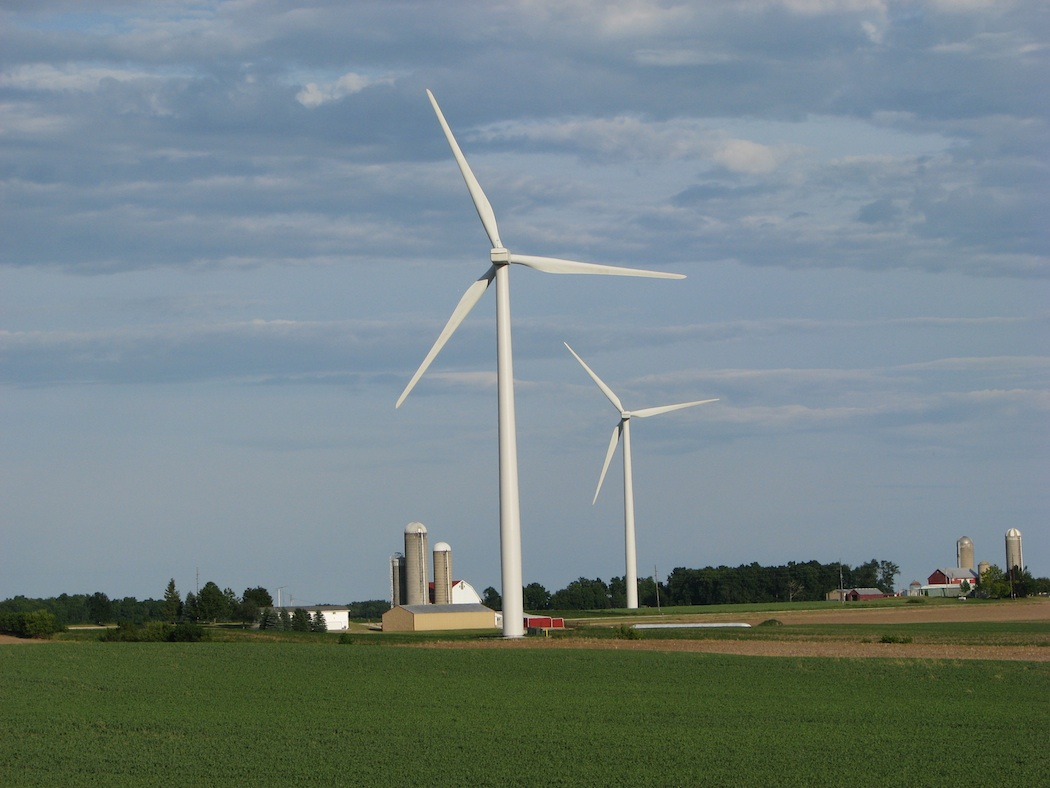
\includegraphics[height=2.5in]{files/21206}
            \caption{Wind turbines at the Forward Wind Energy Center in Fond du Lac and Dodge Counties, Wisconsin. (Photo by Ruth Baranowski / NREL)}\label{fig:21206}
          \end{subfigure}%
          \begin{subfigure}[b]{.5\linewidth}
            \centering
            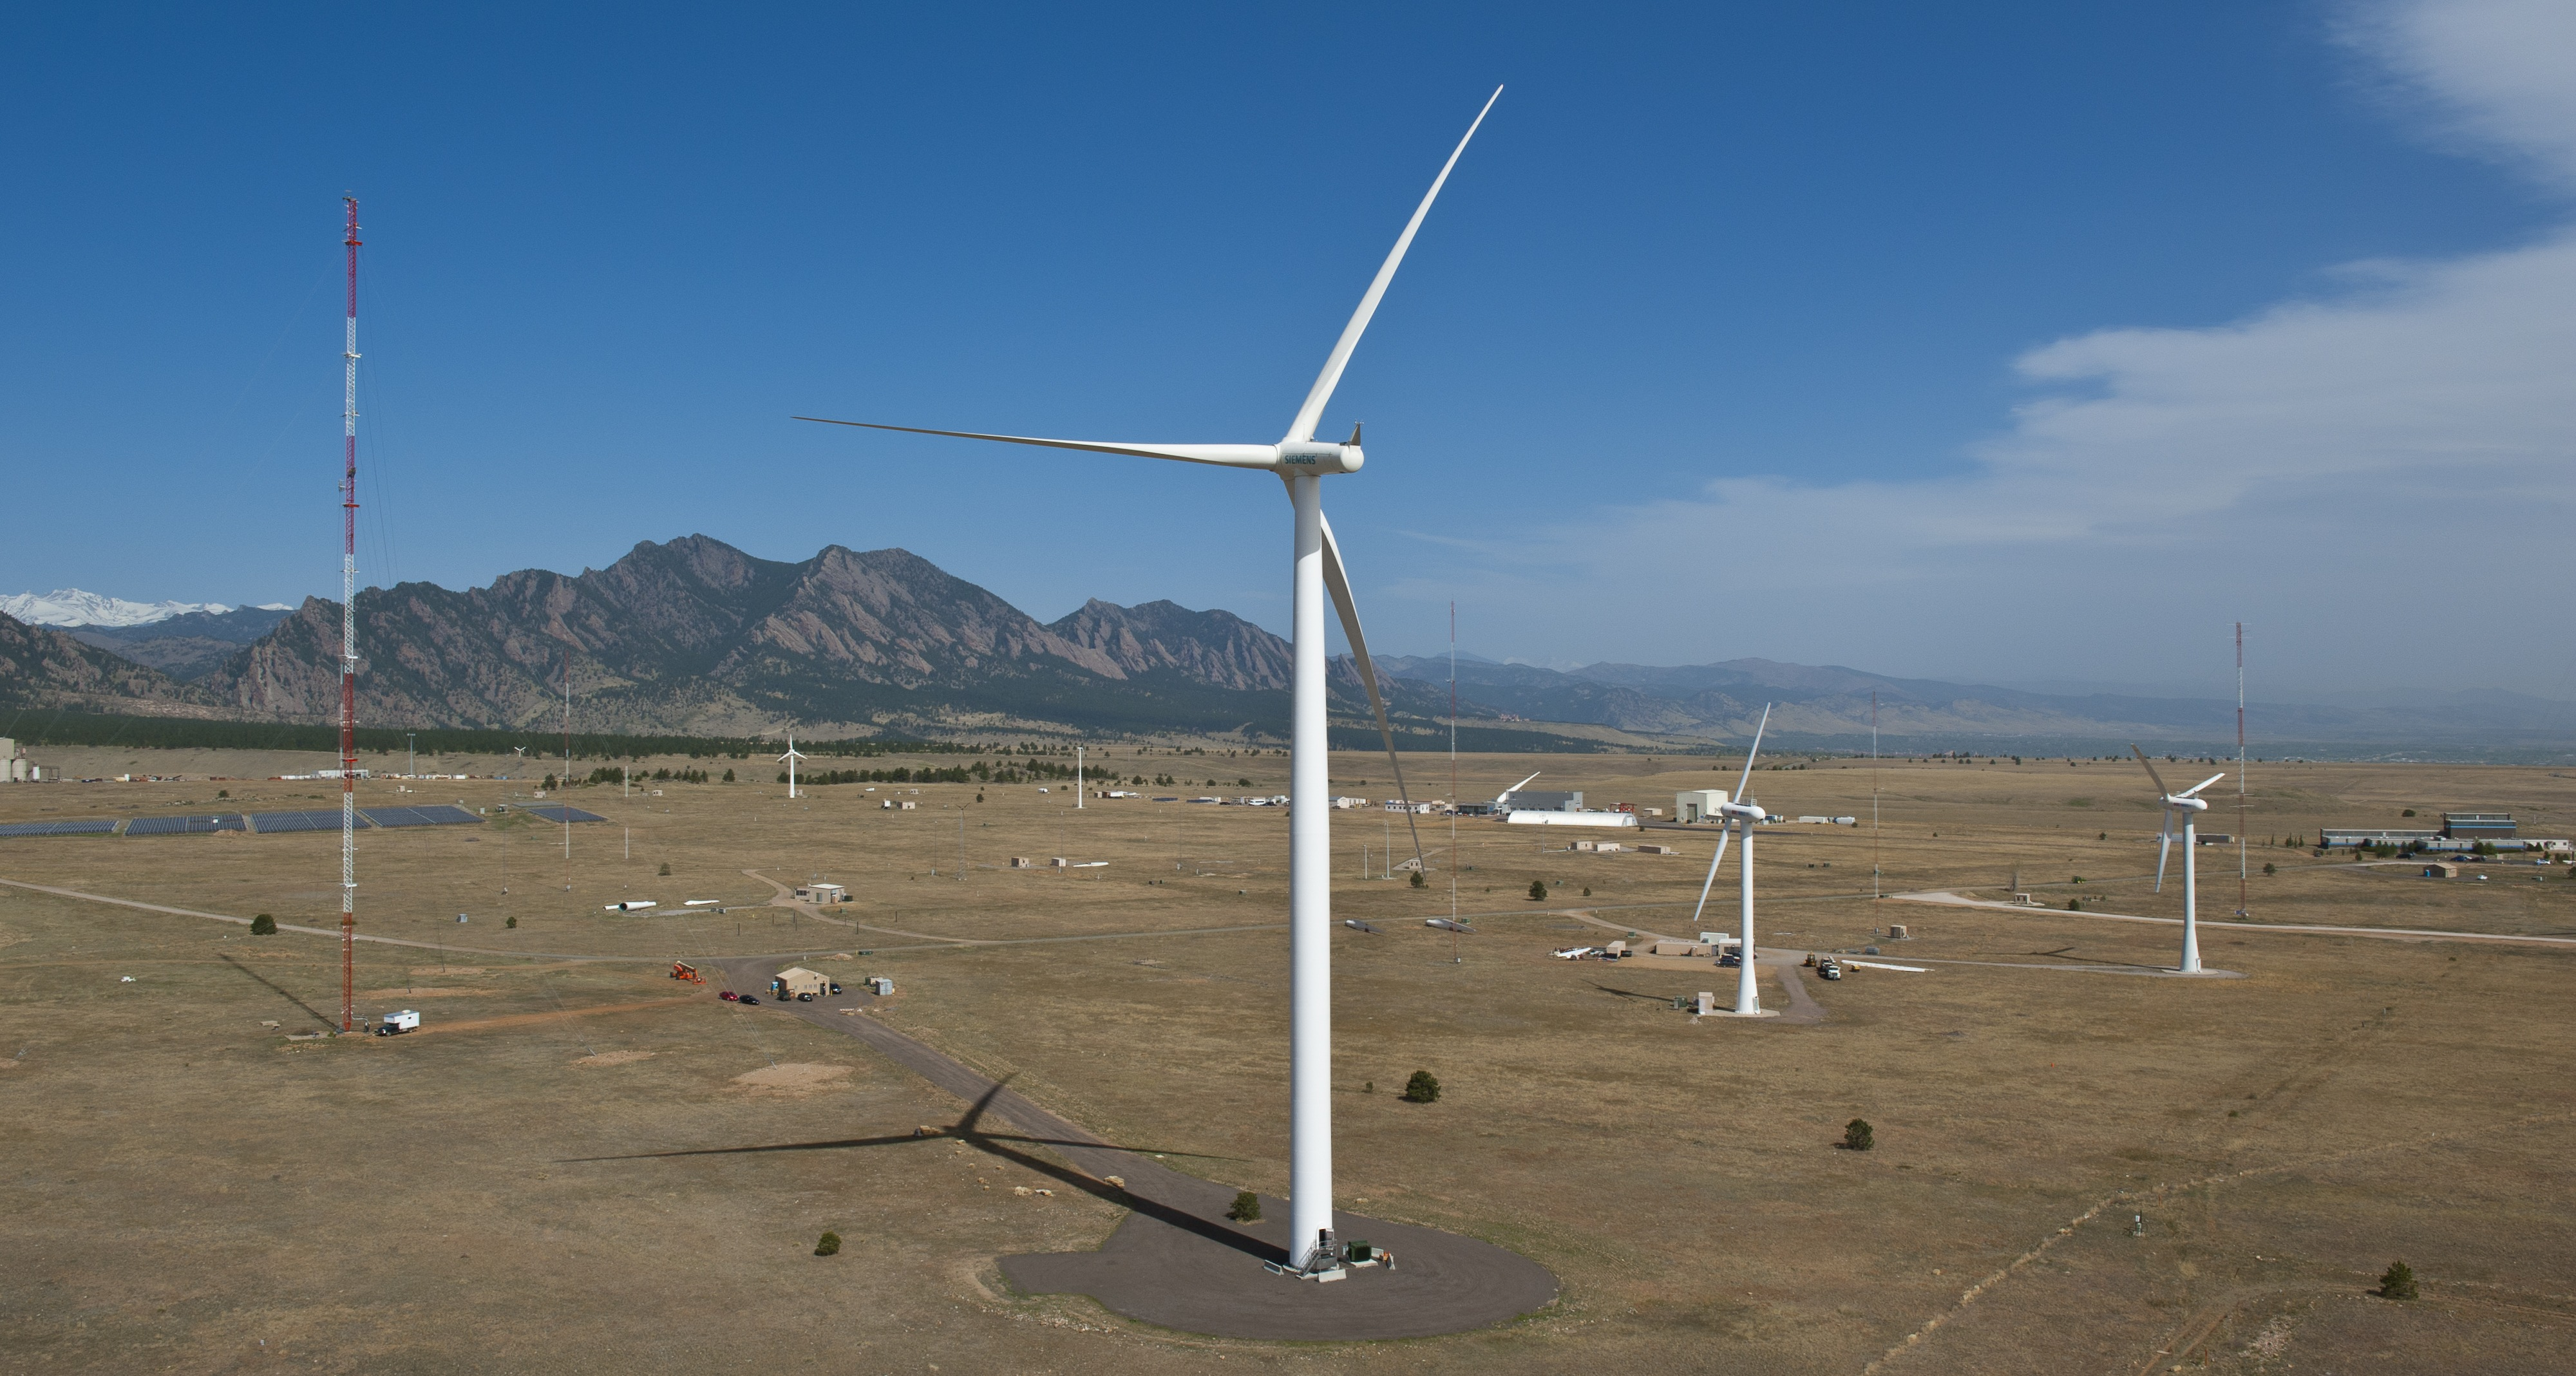
\includegraphics[height=2.5in]{files/20018}
            \caption{Aerial view of the National Wind Technology Center. (Photo by Dennis Schroeder / NREL)}\label{fig:20018}
          \end{subfigure}
          \caption{Images}\label{fig:NRELimages}
\end{figure}
\end{lstlisting}

Note that the \texttt{subfig} and \texttt{subfigure} packages are deprecated. The \texttt{subcaption} package appears to be the most frequently maintained package at this time, and contains the same functionality as the \texttt{subfig} and \texttt{subfigure} packages.

\begin{figure*}
          \begin{subfigure}[t]{.55\linewidth}
            \centering
            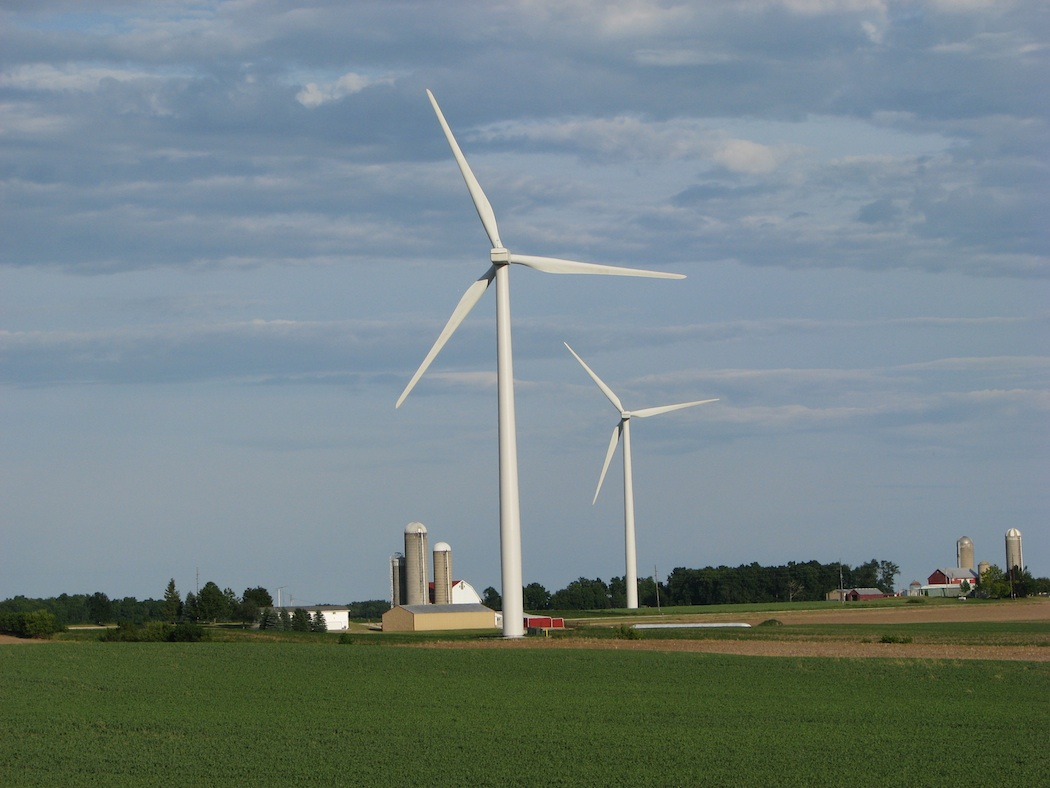
\includegraphics[height=2.5in]{files/21206}
            \caption{Wind turbines at the Forward Wind Energy Center in Fond du Lac and Dodge Counties, Wisconsin. (Photo by Ruth Baranowski / NREL)}\label{fig:21206}
          \end{subfigure}%
          \begin{subfigure}[t]{.55\linewidth}
            \centering
            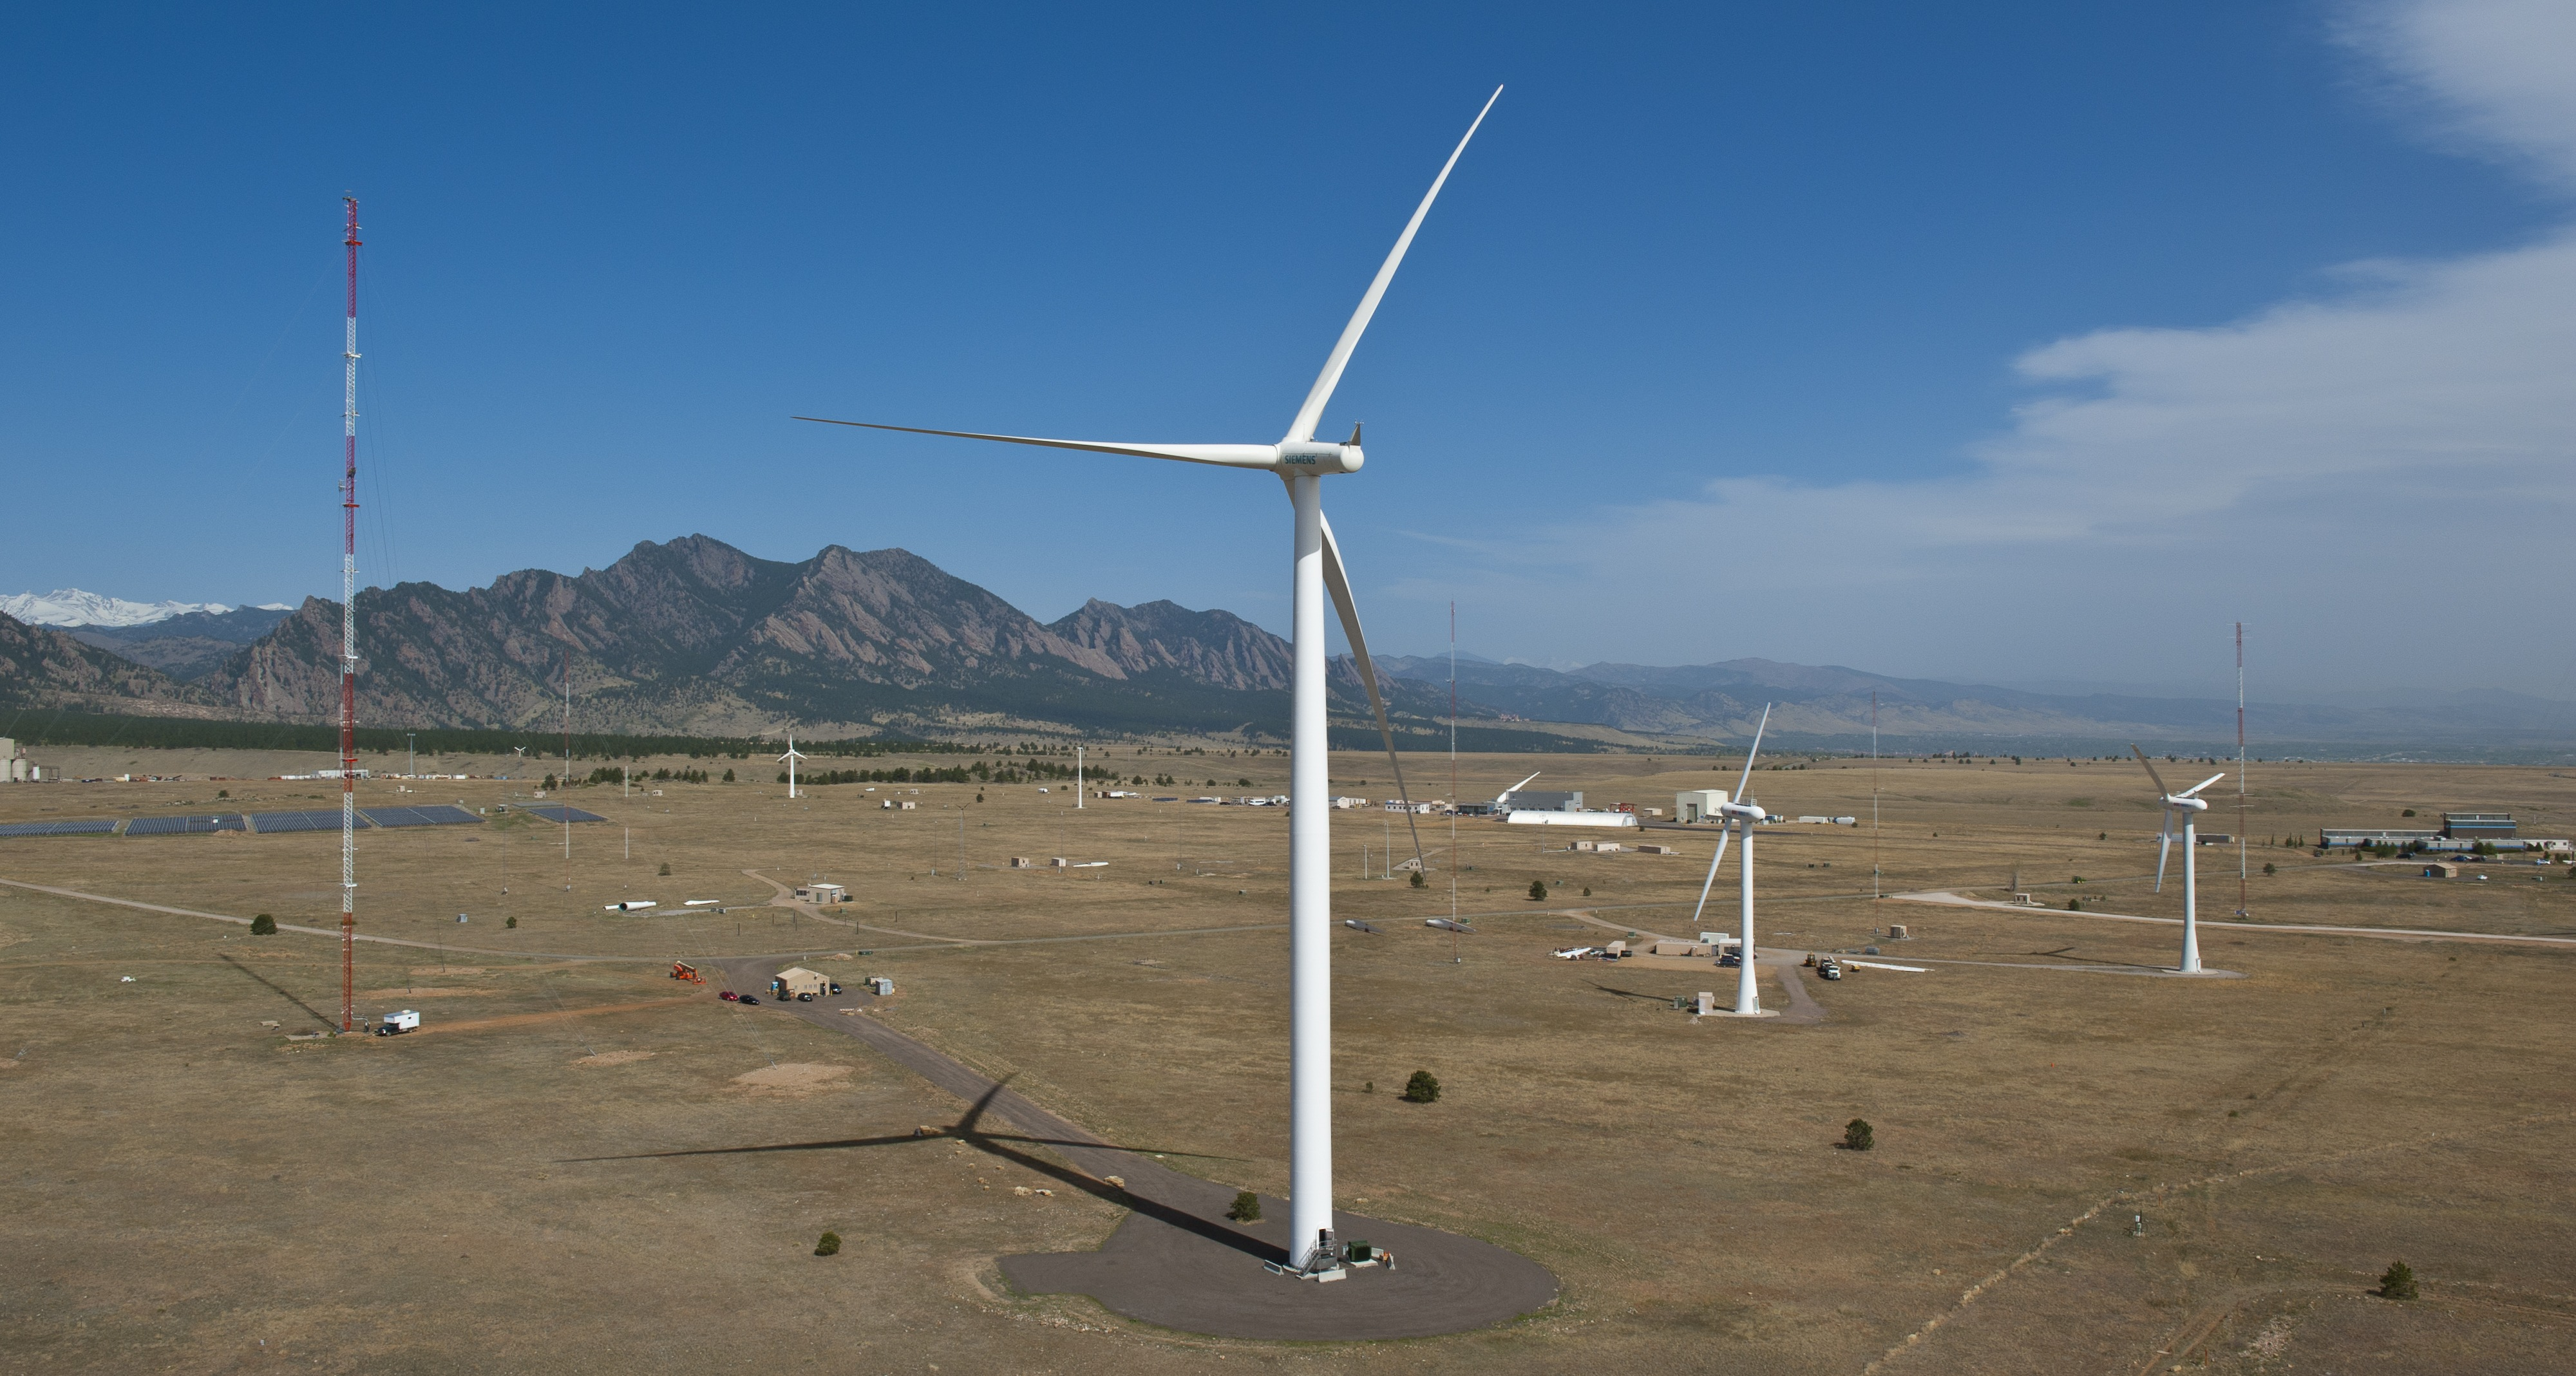
\includegraphics[height=2.5in]{files/20018}
            \caption{Aerial view of the National Wind Technology Center. (Photo by Dennis Schroeder / NREL)}\label{fig:20018}
          \end{subfigure}
          \caption{Images}\label{fig:NRELimages}
\end{figure*}

\subsubsection{Citations}
\label{Sec:Bib}
Use \texttt{bibtex} to organize references and store them in a single file (e.g. \verb+/Documents/bibliography/bibliography.bib+). The bibliography will then contain entries with `keys' for each source, like \texttt{Lamport\_1986\_a}. 

Authors can then insert citations to this key throughout their document, using different styles of citation. Citations are generated using the \texttt{biblatex} package, which also formats references in the correct style.  Ways to generate citations are described in the \texttt{biblatex} documentation, and include:
\begin{itemize}
\item \verb+\cite{Lamport_1986_a}+ prints \cite{Lamport_1986_a}.
\item \verb+\citep{Lamport_1986_a}+ prints \citep{Lamport_1986_a}.
\item \verb+\citet{Lamport_1986_a}+ prints \citet{Lamport_1986_a}.
\end{itemize}

To cite URLs, use the 'misc' style. For example, the bibtex entry for \href{http://tex.stackexchange.com}{http://tex.stackexchange.com}\ \cite{texstackexchange} looks like this:

\begin{lstlisting}
@misc{texstackexchange,
	Author = {Anon.},
	Howpublished = {Accessed July 21, 2014: \url{http://tex.stackexchange.com}},
	Title = {\TeX -- LaTeX Stack Exchange},
	Year = {2014}}
\end{lstlisting}

This format will allow you to include the date on which a URL was accessed.

The citations should work with journal articles \citep{Clifton_2013_a}, books \citep{Knuth_1984_a, Lamport_1986_a, chicago}, technical reports \citep{TechReportTest}, and URLs \citep{texstackexchange}. Any unknown publication types will be formatted using the `misc' type.

\subsubsection{Including computer code}
The \texttt{listings} package has been loaded. Note: this does not work if the `Draft' document option is used.

To change the syntax highlighting use \verb+\lstset{language=[dialect]language, columns=fullflexible, keepspaces=true}+ before each listing where the language changes. For more details see the \texttt{lstlisting} documentation.

\subsubsection{Bibliographies}
This document class uses "Chicago A" style-references produced using Biblatex. The reference style can be changed in the \emph{CorporateArticle.cls} file.

To include a bibliography in the document give the bibliography file location in the preamble and insert the bibliography at the appropriate location:

\begin{lstlisting}
% give the bibliography file location
\bibliography{files/bibliography.bib}
...
\begin{document}
...
% insert the bibliography into the document
\cleardoublepage
\label{sec:Bib}
\printbibliography
...
\end{document}
\end{lstlisting}

An example bibliography is included in this document on page \pageref{sec:Bib}.

\subsubsection{Footnotes}
Footnotes can be inserted using the \verb+\footnote{}+ command\footnote{like this}. Footnotes are numbered in the main matter\footnote{and like this as well}, and use daggers, etc instead of numers in the appendices.

\subsection{Creating a file structure}
\label{sec:FileStructure}
Your main file should be called \emph{main.tex}. This helps editors and coauthors identify where to start. Then, use \texttt{input} to import other files into your main file at compilation.

For example, each of the chapters in this report is in separate files, called \emph{WhatIsLatex} (Chapter 1), \emph{LatexForDocs} (Chapter 2), and so-on. In the example available on Github, they are stored in the \emph{files} directory. \emph{main.tex} then looks like this:

\begin{lstlisting}
...
\begin{document}
% content
\input{files/WhatIsLatex}
\input{files/LatexForDocs}
...
\end{lstlisting}

\subsection{Best practice in writing a document in LaTeX}
\begin{description}
\item[Create a structure before you get too far.] Authors will find it easier to write documents and make changes if they separate the content of the document from the structure.
\begin{enumerate}
\item Each new LaTeX document should be placed in it's own directory. 
\item Create a main LaTeX file that just contains the preamble, custom commands and uses \texttt{input} to call the content. See Section \ref{sec:FileStructure} for an example where each \texttt{chapter} is contained in its own file. In an article, each \texttt{section} could be contained in its own file.
\item Keep the number of packages used to a minimum. Not all packages can be used as they lack compatibility.
\end{enumerate}
\item[Focus on content, not appearance.] Don't spend hours trying to adjust fonts, headers or spacing between lines. 
\begin{enumerate}
\item Don't throw in lots of \texttt{clearpage}s or other commands to push material around. LaTeX is designed to handle that. 
\item Resist the temptation to add or subtract space, change lengths or do other things to modify the layout. 
\item Write!
\end{enumerate}
\end{description}

...
\end{lstlisting}

\subsection{Best practice in writing a document in LaTeX}
\begin{description}
\item[Create a structure before you get too far.] Authors will find it easier to write documents and make changes if they separate the content of the document from the structure.
\begin{enumerate}
\item Each new LaTeX document should be placed in it's own directory. 
\item Create a main LaTeX file that just contains the preamble, custom commands and uses \texttt{input} to call the content. See Section \ref{sec:FileStructure} for an example where each \texttt{chapter} is contained in its own file. In an article, each \texttt{section} could be contained in its own file.
\item Keep the number of packages used to a minimum. Not all packages can be used as they lack compatibility.
\end{enumerate}
\item[Focus on content, not appearance.] Don't spend hours trying to adjust fonts, headers or spacing between lines. 
\begin{enumerate}
\item Don't throw in lots of \texttt{clearpage}s or other commands to push material around. LaTeX is designed to handle that. 
\item Resist the temptation to add or subtract space, change lengths or do other things to modify the layout. 
\item Write!
\end{enumerate}
\end{description}

...
\end{lstlisting}

\subsection{Best practice in writing a document in LaTeX}
\begin{description}
\item[Create a structure before you get too far.] Authors will find it easier to write documents and make changes if they separate the content of the document from the structure.
\begin{enumerate}
\item Each new LaTeX document should be placed in it's own directory. 
\item Create a main LaTeX file that just contains the preamble, custom commands and uses \texttt{input} to call the content. See Section \ref{sec:FileStructure} for an example where each \texttt{chapter} is contained in its own file. In an article, each \texttt{section} could be contained in its own file.
\item Keep the number of packages used to a minimum. Not all packages can be used as they lack compatibility.
\end{enumerate}
\item[Focus on content, not appearance.] Don't spend hours trying to adjust fonts, headers or spacing between lines. 
\begin{enumerate}
\item Don't throw in lots of \texttt{clearpage}s or other commands to push material around. LaTeX is designed to handle that. 
\item Resist the temptation to add or subtract space, change lengths or do other things to modify the layout. 
\item Write!
\end{enumerate}
\end{description}

%% CHAPTER: MAKING PDFS
\chapter{Preparing a high-quality PDF from LaTeX}\label{sec:PDFprep}
If the author chooses to complete the publications process using LaTeX\, the author must incorporate feedback and edits in to the LaTeX source files and prepare the final PDF, following these guidelines.

\section{PDF tagging}\label{sec:PDFtagging}
PDF tagging is a process whereby the components of the PDF document (headings, figures, tables, text) are marked so that a document reader can understand the document. This is useful when text to speech converters are being used. The process of tagging is also known as structuring, so that a tagged document might also be referred to as a structured document.

LaTeX does not prepare a tagged PDF document. The current solution to this is to use the tagging capability built in to Adobe's Acrobat Pro.

To prepare a tagged document, follow these steps:
\begin{enumerate}
\item Add tags. Go to the `Advanced' menu. Select `Accessibility', then `Add tags to document'.
\item Add alternative text for figures. Context-click the Figure, select `Properties', and fill in `Alternate Text'. Alternatively, try the process outlined below.
\item Specify the document language. Go to the `File' menu. Select `Document Properties', then the `Advanced' tab, `Language' field. In some versions of Acrobat, the sequence is `File', `Properties', `Reading Options', `Language'.
\item Define tab order.
\begin{enumerate}
\item Go to the `View' menu. Select `Navigation tabs', then `Pages'.
\item Click on any page, then type Ctrl-A (or Command-A on a Mac) to select all the pages.
\item Go to the `Options' menu in the top right of the dialog box, and select `Page Properties'
\item In the `Tab Order' tab, select `Use document structure'.
\end{enumerate}
\item Make sure tables have headings. 
\begin{enumerate}
\item Go to the `View' menu. Select `Navigation tabs', then `Tags'.
\item Select the `Tags' tab. This panel shows the document structure as a tree.
\item Navigate to the table cells that should be headers.
\item Check they have the type <TH>. If not, then right click on the header cell, select `properties', select the `Tag' tab, and change the value for `Type' to <TH>.
\end{enumerate}
\item Make sure all Chapters (or sections, if there are no chapters in the document) are correctly tagged.
\end{enumerate}

\section{Alt-text on images and equations}
`Alt text' is a textual description of an equation, link or figure. The following short equation should pop-up some text when a user passes a mouse over it. This should work in most PDF readers:
\begin{equation}
\pdftooltip{a^2+b^2=c^2}{An equation}
%a^2+b^2=c^2
\end{equation}

The alt text can be added after the PDF is compiled, or written in to the source document. The rest of this section describes how it can be added to the source and generated by LaTeX using the \href{pdfcomment}{http://www.ctan.org/pkg/pdfcomment} package. The general form of the command is:

\begin{verbatim}
\pdftooltip{<item>}{<pop-up text>}
\end{verbatim}

The previous equation was generated using this code:

\begin{verbatim}
\begin{equation}
\pdftooltip{a^2+b^2=c^2}{An equation}
\end{equation}
\end{verbatim}

The same approach can be used to create alt-text for images. For example, Figure \ref{fig:NRELimagesWithAltText} has been labeled. The code for this image is:

\begin{verbatim}
\begin{figure}[!h]
\centering
\hfill
\subfigure[Wind turbines at the Forward Wind Energy Center in Fond du Lac and Dodge Counties, Wisconsin. (Photo by Ruth Baranowski / NREL)] {\pdftooltip{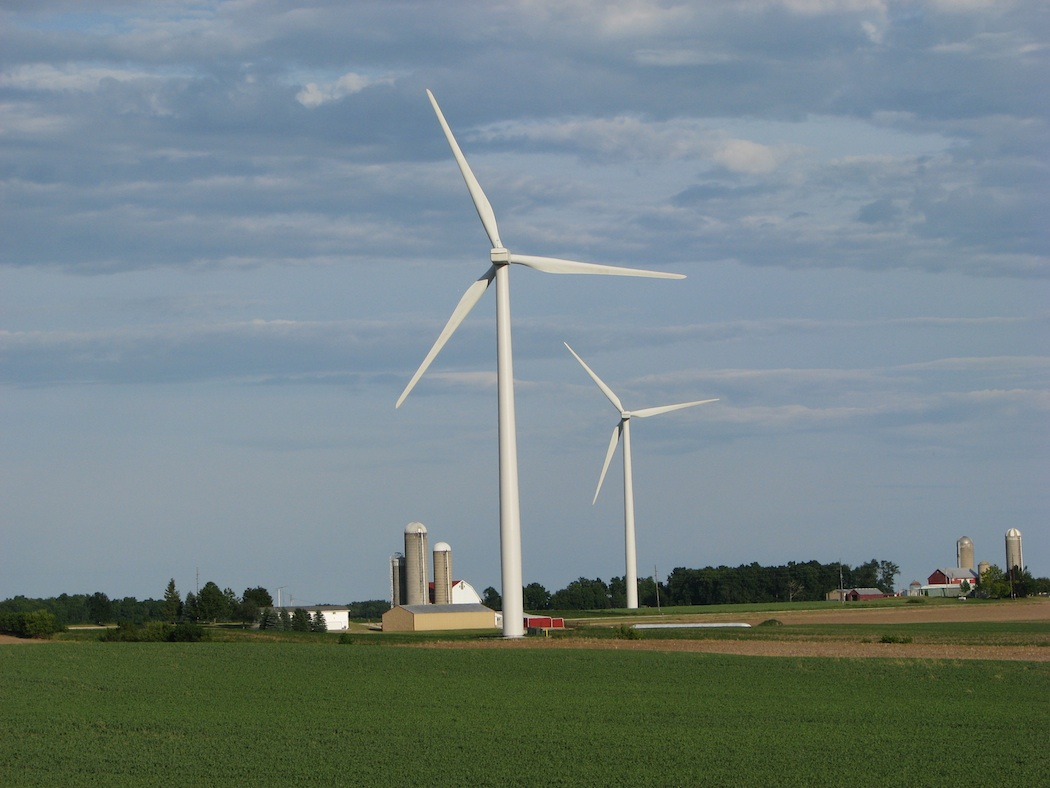
\includegraphics[height=2.5in]{files/21206}}{This is an image}}
~ 
\hfill
\subfigure[Aerial view of the National Wind Technology Center.  (Photo by Dennis Schroeder / NREL)] {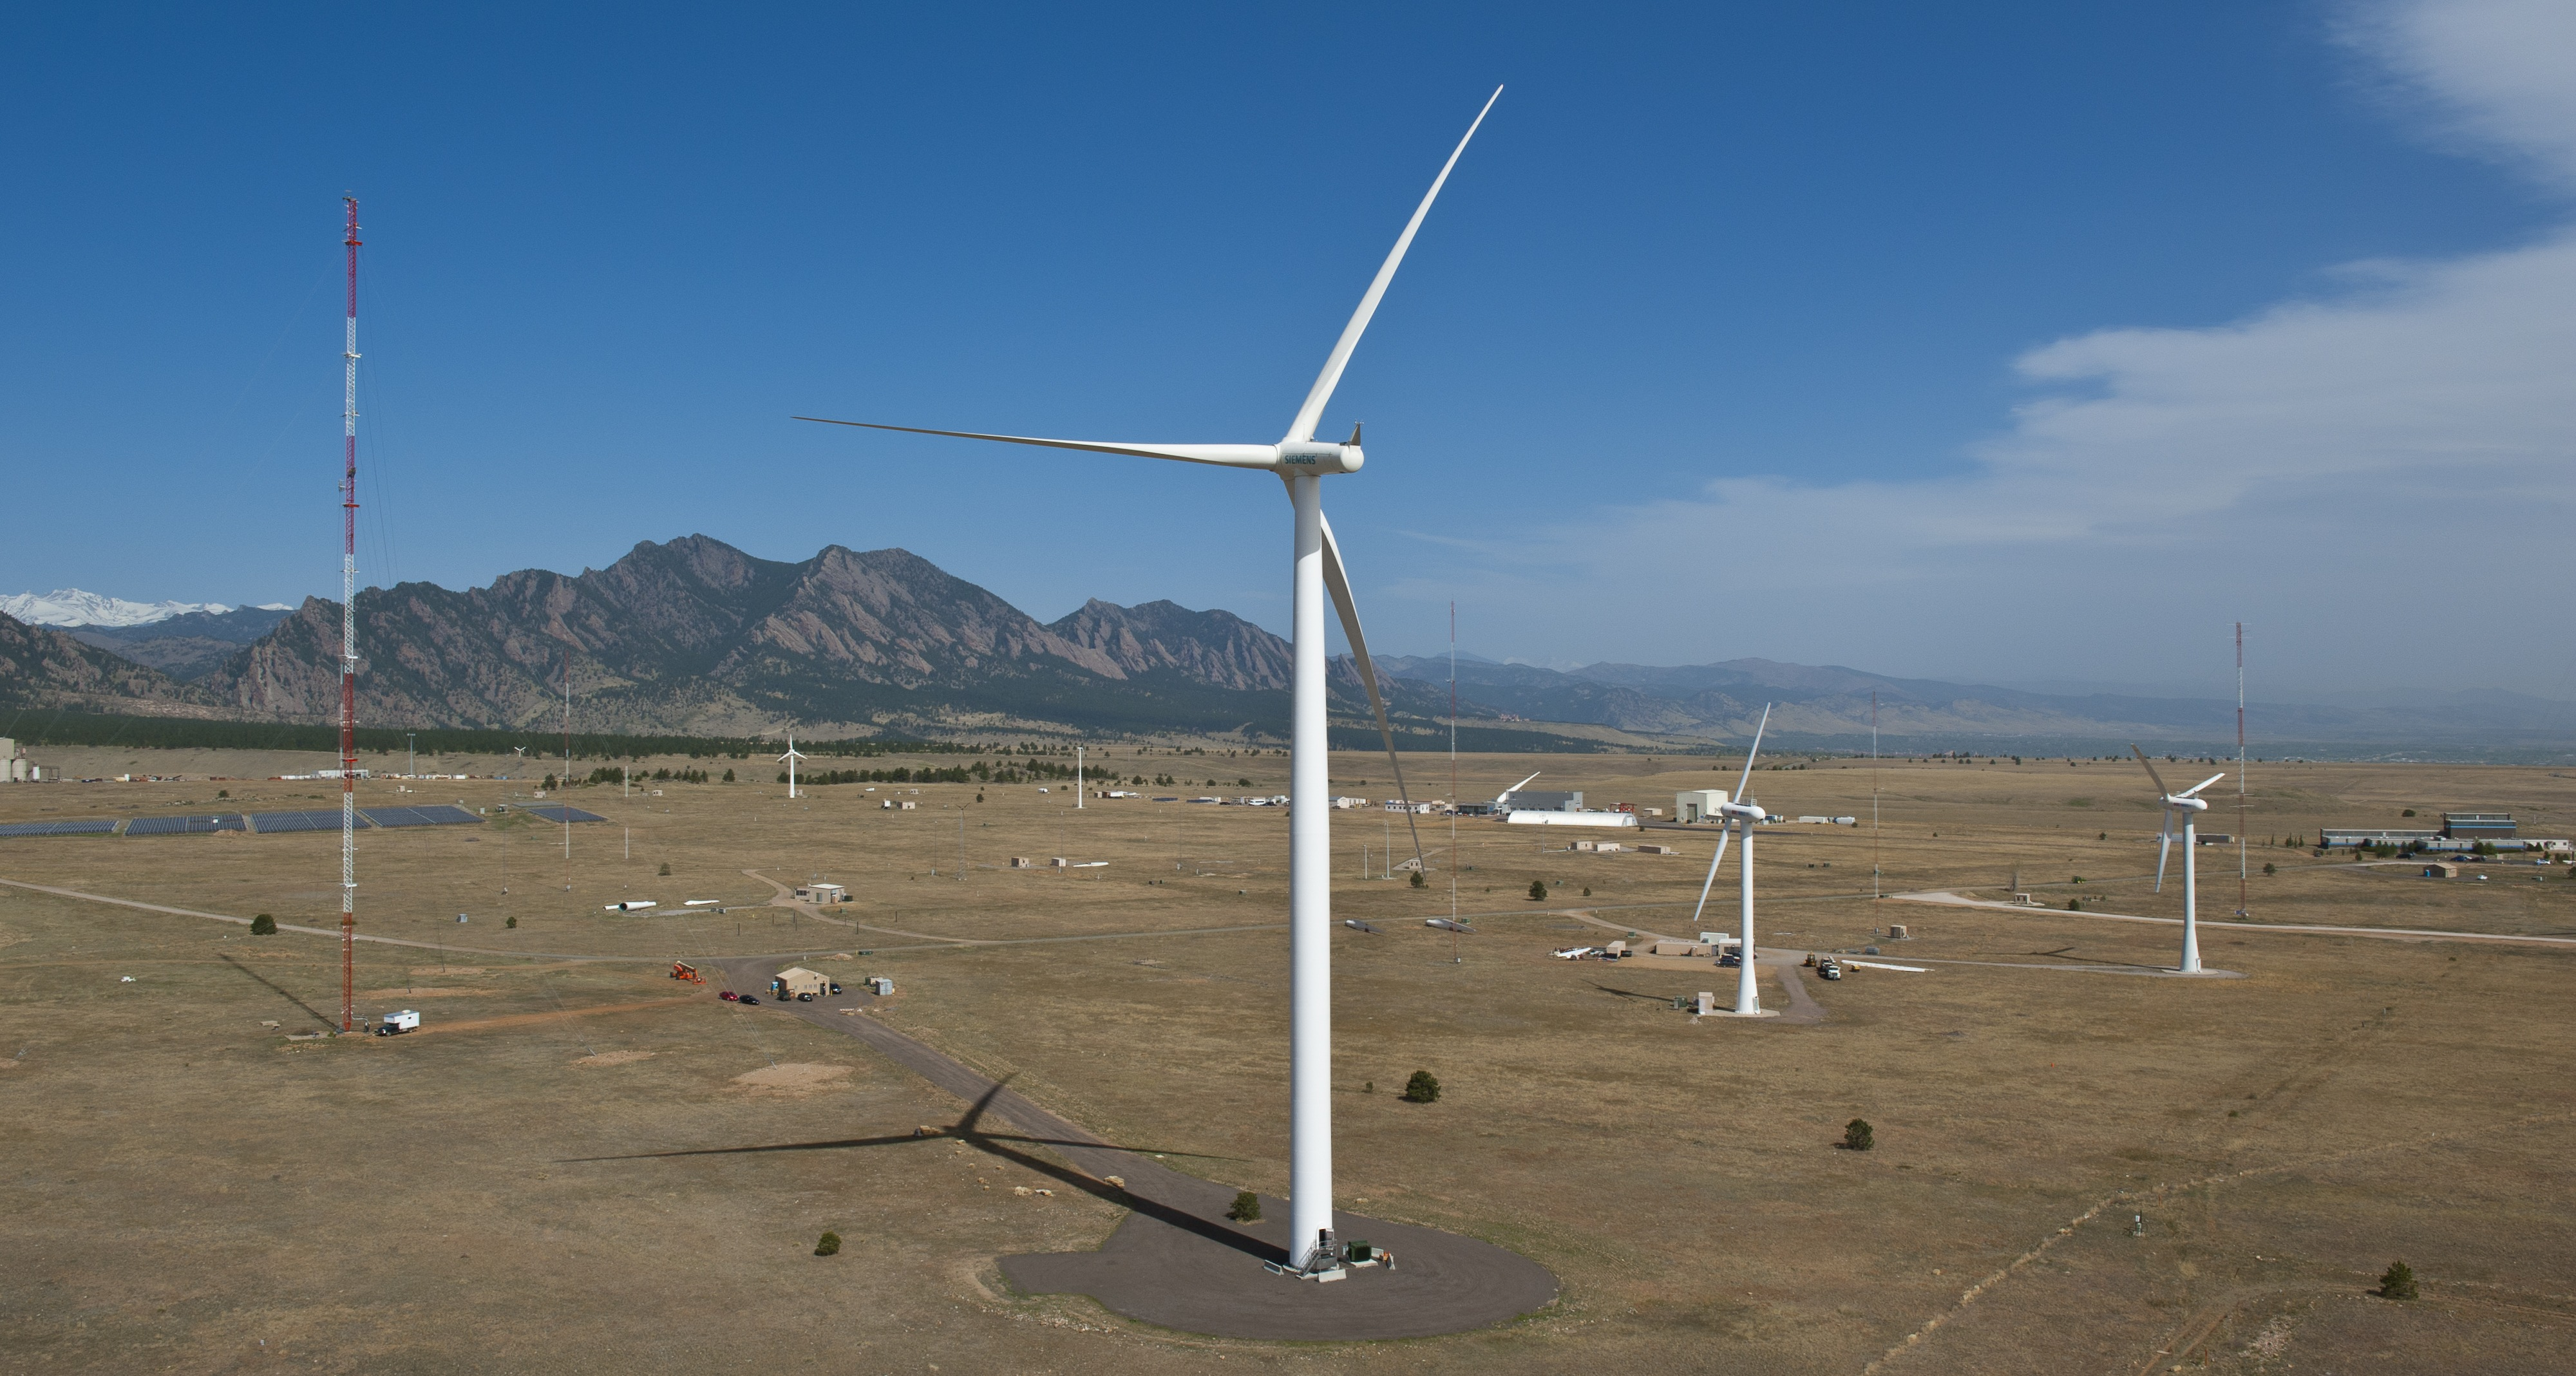
\includegraphics[height=2.5in]{files/20018}}
\hfill
\caption{NREL images}\label{fig:NRELimagesWithAltText}
\end{figure}
\end{verbatim}

\begin{figure}[!h]
\centering
\hfill
\subfigure[Wind turbines at the Forward Wind Energy Center in Fond du Lac and Dodge Counties, Wisconsin. (Photo by Ruth Baranowski / NREL)]{\pdftooltip{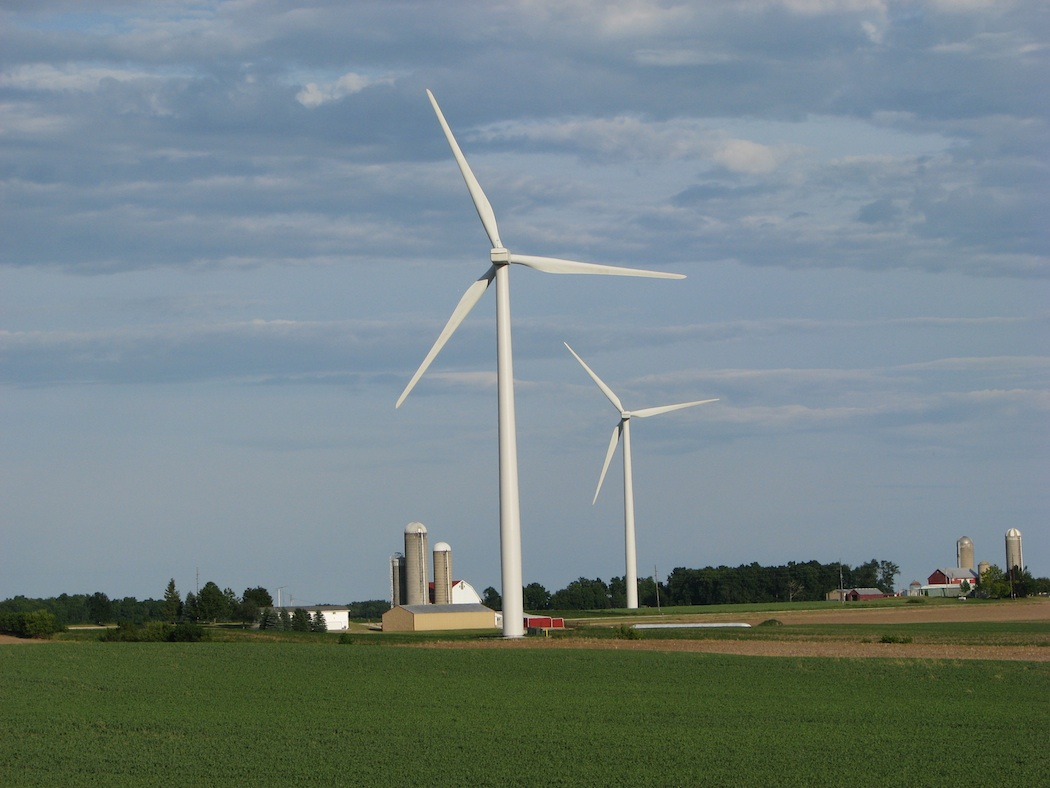
\includegraphics[height=2.5in]{files/21206}}{This is an image. It may be possible to propagate the caption into this text.}}
%{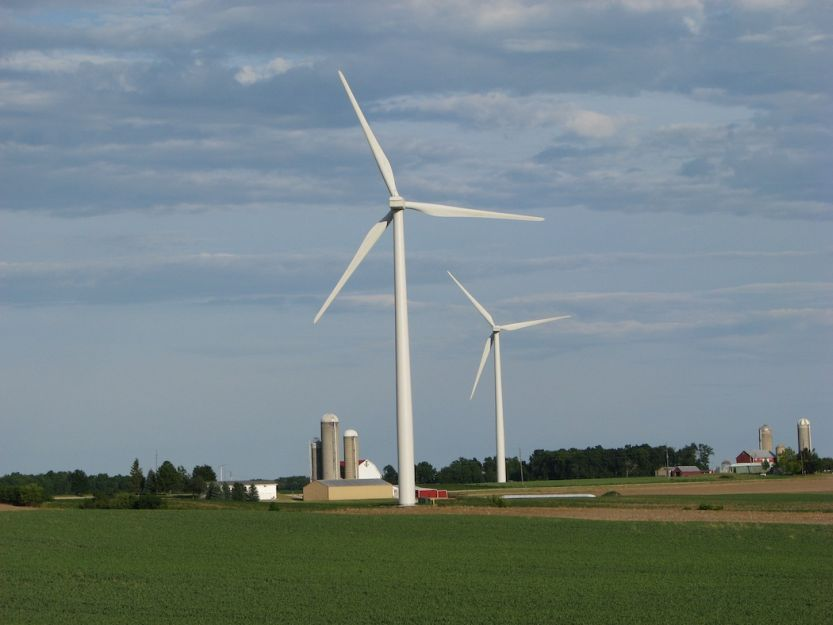
\includegraphics[height=2.5in]{21206}}
~ %add desired spacing between images, e. g. ~, \quad, \qquad etc. (or a blank line to force the subfigure onto a new line)
\hfill
\subfigure[Aerial view of the National Wind Technology Center. (Photo by Dennis Schroeder / NREL)]{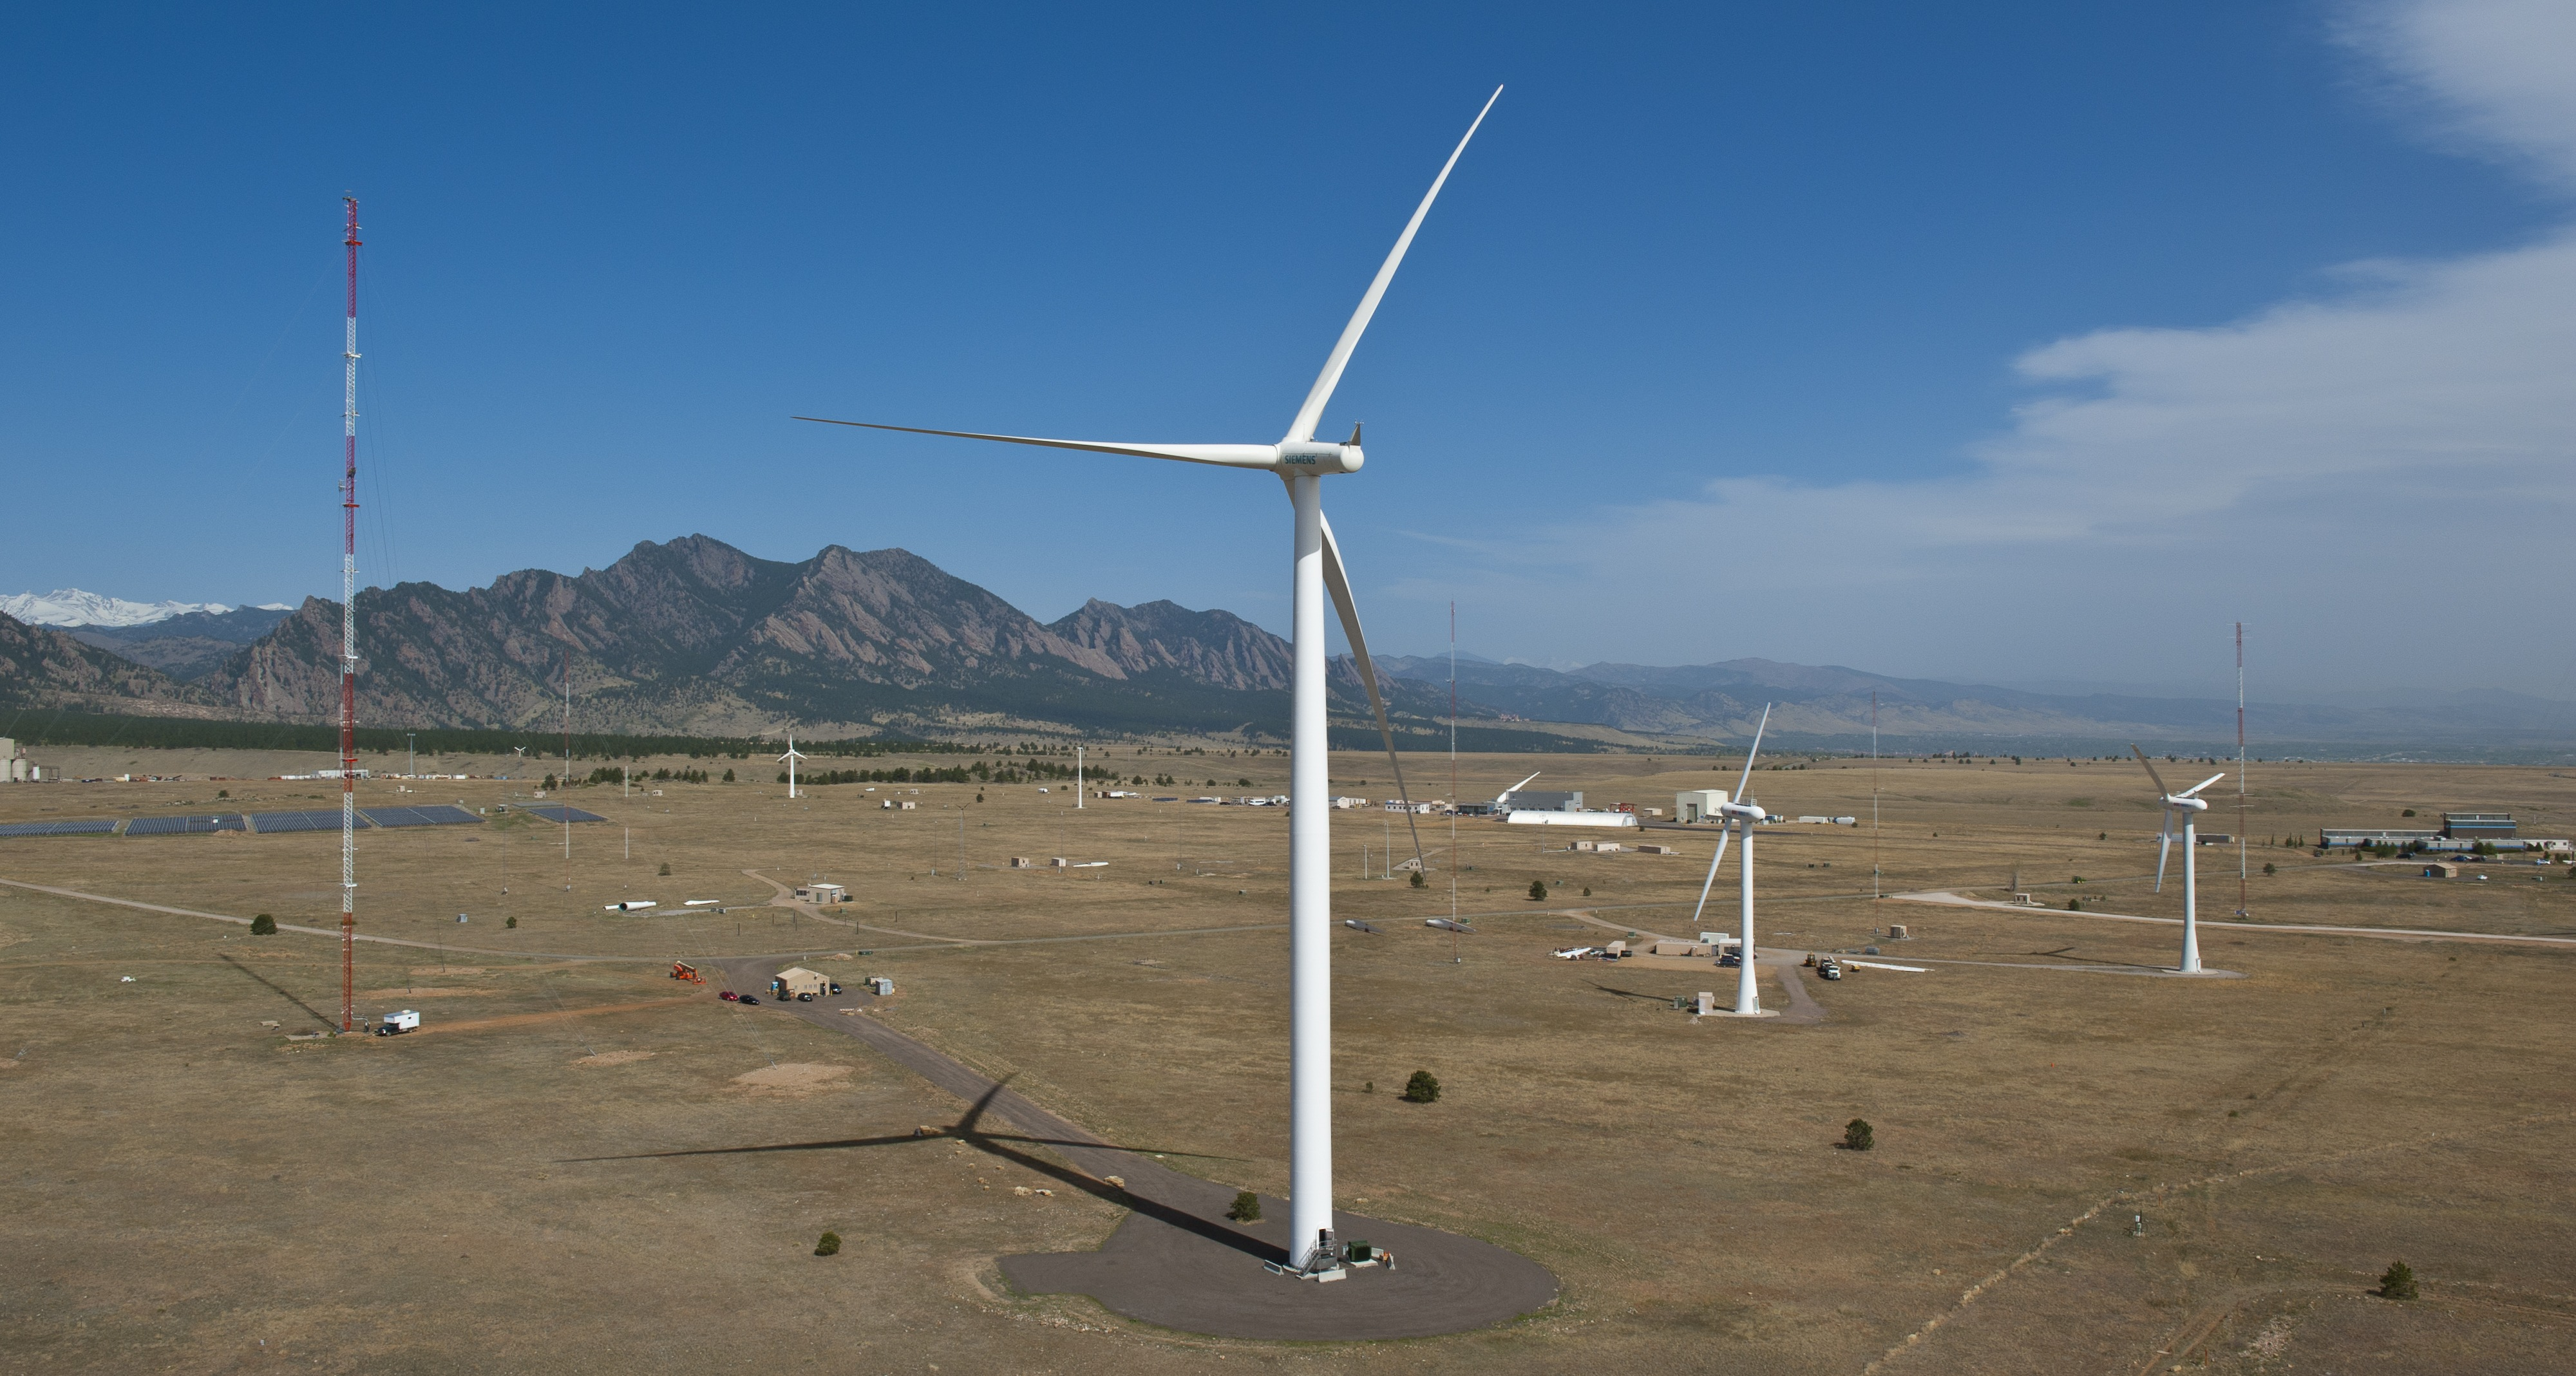
\includegraphics[height=2.5in]{files/20018}}
\hfill
\caption{NREL images}\label{fig:NRELimagesWithAltText}
\end{figure}

Alt-text is not processed by \texttt{latex2rtf}. So, if the author anticipates finishing the publication solely as a .DOC or .DOCX file, they do not need to use alt-text.

\section{Embedded fonts}
NREL requires that all fonts be embedded in the the final PDF. Check the PDF for embedded fonts using a PDF viewer. For example, in Adobe Acrobat Reader, look at the `fonts' tag of the document properties. If any fonts are not shown as being an \emph{embedded subset}, try the conversion again. 

Encapsulated postscript figures are particularly prone to having undefined fonts. Check by compiling the document in draft mode, and seeing if the fonts are still present in the output PDF. To fix this problem, consider changing the \emph{.eps} file to a \emph{.png}. To do this `on the fly', use this in the document's preamble:

\begin{verbatim}
\usepackage{epstopdf}
\epstopdfDeclareGraphicsRule
 {.eps}{png}{.png}{convert eps:\SourceFile.\SourceExt png:\OutputFile}
\AppendGraphicsExtensions{.png}
\end{verbatim}
%% CHAPTER: APPENDICES
\appendix
\section{How to Use Appendices}
Appendices can be included in NREL documents. 

\subsection{How to switch to appendixes}
To switch to appendices, simply use the \emph{appendix} command:

\begin{lstlisting}
\appendix
\section{How to Use Appendices}
Appendices can be included in NREL documents. 

\subsection{How to switch to appendixes}
To switch to appendices, simply use the \emph{appendix} command:

\begin{lstlisting}
\appendix
\section{How to Use Appendices}
Appendices can be included in NREL documents. 

\subsection{How to switch to appendixes}
To switch to appendices, simply use the \emph{appendix} command:

\begin{lstlisting}
\appendix
\input{files/AppendixA}
\input{files/AppendixB}
\end{lstlisting}

\subsection{Changes to Figure, Table, and Footnote Numbering}
The following table (Table \ref{tab:AppAWidgets}) should have a different caption numbering style than Table \ref{tab:widgets}. The table number should start with the appendix label (in this case \thesection,) be followed by a period, and then be numbered. Numbering should restart in each new appendix.

\begin{table}[!h]
\centering
\caption{An example table.}\label{tab:AppAWidgets}
\begin{tabular}{lr}
Item & Quantity \\
\hline
Widgets & 42 \\
Gadgets & 13
\end{tabular}
\end{table}

The following table should use the same letter as Table \ref{tab:AppAWidgets}, but the number should be incremented by one.

\begin{table}[!h]
\centering
\caption{An example table.}\label{tab:AppAWidgetsTwo}
\begin{tabular}{lr}
Item & Quantity \\
\hline
Widgets & 42 \\
Gadgets & 13
\end{tabular}
\end{table}

Footnotes use symbols in place of numbers in the appendices\footnote{this is a test}.
\section{Including Multiple Appendices}
This chapter is included to demonstrate that the \emph{nrel.cls} file correctly formats a second appendix\footnote{this is also a test}.

\subsection{Changes to numbering}
The following table (Table \ref{tab:AppBWidgets}) caption should have a different numbering style than Table \ref{tab:widgets}. Instead, the caption numbering style should be the same as Table \ref{tab:AppAWidgets}. Numbering in this chapter should start with \thesection.

\begin{table}[!h]
\centering
\caption{An example table.}\label{tab:AppBWidgets}
\begin{tabular}{lr}
Item & Quantity \\
\hline
Widgets & 42 \\
Gadgets & 13
\end{tabular}
\end{table}

\end{lstlisting}

\subsection{Changes to Figure, Table, and Footnote Numbering}
The following table (Table \ref{tab:AppAWidgets}) should have a different caption numbering style than Table \ref{tab:widgets}. The table number should start with the appendix label (in this case \thesection,) be followed by a period, and then be numbered. Numbering should restart in each new appendix.

\begin{table}[!h]
\centering
\caption{An example table.}\label{tab:AppAWidgets}
\begin{tabular}{lr}
Item & Quantity \\
\hline
Widgets & 42 \\
Gadgets & 13
\end{tabular}
\end{table}

The following table should use the same letter as Table \ref{tab:AppAWidgets}, but the number should be incremented by one.

\begin{table}[!h]
\centering
\caption{An example table.}\label{tab:AppAWidgetsTwo}
\begin{tabular}{lr}
Item & Quantity \\
\hline
Widgets & 42 \\
Gadgets & 13
\end{tabular}
\end{table}

Footnotes use symbols in place of numbers in the appendices\footnote{this is a test}.
\section{Including Multiple Appendices}
This chapter is included to demonstrate that the \emph{nrel.cls} file correctly formats a second appendix\footnote{this is also a test}.

\subsection{Changes to numbering}
The following table (Table \ref{tab:AppBWidgets}) caption should have a different numbering style than Table \ref{tab:widgets}. Instead, the caption numbering style should be the same as Table \ref{tab:AppAWidgets}. Numbering in this chapter should start with \thesection.

\begin{table}[!h]
\centering
\caption{An example table.}\label{tab:AppBWidgets}
\begin{tabular}{lr}
Item & Quantity \\
\hline
Widgets & 42 \\
Gadgets & 13
\end{tabular}
\end{table}

\end{lstlisting}

\subsection{Changes to Figure, Table, and Footnote Numbering}
The following table (Table \ref{tab:AppAWidgets}) should have a different caption numbering style than Table \ref{tab:widgets}. The table number should start with the appendix label (in this case \thesection,) be followed by a period, and then be numbered. Numbering should restart in each new appendix.

\begin{table}[!h]
\centering
\caption{An example table.}\label{tab:AppAWidgets}
\begin{tabular}{lr}
Item & Quantity \\
\hline
Widgets & 42 \\
Gadgets & 13
\end{tabular}
\end{table}

The following table should use the same letter as Table \ref{tab:AppAWidgets}, but the number should be incremented by one.

\begin{table}[!h]
\centering
\caption{An example table.}\label{tab:AppAWidgetsTwo}
\begin{tabular}{lr}
Item & Quantity \\
\hline
Widgets & 42 \\
Gadgets & 13
\end{tabular}
\end{table}

Footnotes use symbols in place of numbers in the appendices\footnote{this is a test}.
\section{Including Multiple Appendices}
This chapter is included to demonstrate that the \emph{nrel.cls} file correctly formats a second appendix\footnote{this is also a test}.

\subsection{Changes to numbering}
The following table (Table \ref{tab:AppBWidgets}) caption should have a different numbering style than Table \ref{tab:widgets}. Instead, the caption numbering style should be the same as Table \ref{tab:AppAWidgets}. Numbering in this chapter should start with \thesection.

\begin{table}[!h]
\centering
\caption{An example table.}\label{tab:AppBWidgets}
\begin{tabular}{lr}
Item & Quantity \\
\hline
Widgets & 42 \\
Gadgets & 13
\end{tabular}
\end{table}



% bibliography
\cleardoublepage
\label{sec:Bib}
\printbibliography[heading=bibintoc]
\end{document}